\documentclass[a4paper,landscape,7pt,fleqn]{scrartcl}
\usepackage[english]{babel}
\usepackage[utf8]{inputenc}
\usepackage[a4paper, landscape, margin=1.1cm]{geometry}
\usepackage{fullpage}
\usepackage{latexsym}
\usepackage{multicol}
\usepackage{amsmath}
\usepackage{amsfonts}
\usepackage{amssymb}
\usepackage{mathtools}
\usepackage{array}
\usepackage{graphicx}
\usepackage{booktabs}
\usepackage{float}			% add H as an option for floats
\usepackage{parskip}		% add no indentation to new paragraphs
\usepackage{empheq}		% emphasize (box) equations
\usepackage{enumitem}	% description lists
\usepackage{fancyhdr}
\usepackage{lastpage}
\usepackage{framed}

\typearea{16}
\pagestyle{plain}
\columnsep 30pt
\columnseprule .4pt

\newcommand*\widefbox[1]{\fbox{\hspace{2em}#1\hspace{2em}}}		% required for boxing several lines of equations at once

\renewcommand*{\familydefault}{\sfdefault}		% set font to default sans-serif

\renewcommand{\labelitemi}{\tiny$\blacksquare$}		% change symbol of itemized lists
\setlist[itemize]{leftmargin=0.4cm}								% reduce indentation of itemized lists

\renewcommand{\arraystretch}{1}
\renewcommand{\emph}[1]{\textbf{#1}}

\graphicspath{ {images/} }

\pagestyle{fancy}
\fancyhead{}
\setlength{\headheight}{0pt}
\setlength{\footheight}{14pt}
\renewcommand{\headrulewidth}{0pt}
\renewcommand{\footrulewidth}{0.5pt}
\lfoot{Fabian MARBACH}
\cfoot{p \thepage\ / \pageref{LastPage}}
\rfoot{Financial Engineering}

%\allowdisplaybreaks	% equations can be split on two pages/columns

\usepackage{parskip}	% add no indentation to new paragraphs

\makeatletter
\renewcommand{\section}{\@startsection{section}{1}{0mm}%
{-2\baselineskip}{0.8\baselineskip}%
{\hrule depth 0.2pt width\columnwidth\hrule depth1.5pt
width0.25\columnwidth\vspace*{1.2em}\Large\bfseries}}
\makeatother

\makeatletter
\renewcommand{\subsection}{\@startsection{subsection}{1}{0mm}%
{-2\baselineskip}{0.8\baselineskip}%
{\hrule depth 0.2pt width\columnwidth\hrule depth0.75pt
width0.25\columnwidth\vspace*{1.2em}\large\bfseries}}
\makeatother

\makeatletter
\renewcommand{\subsubsection}{\@startsection{subsubsection}{1}{0mm}%
{-2\baselineskip}{0.8\baselineskip}%
{\hrule depth 0.2pt width\columnwidth\vspace*{1.2em}\normalsize\bfseries}}
\makeatother

\newcommand{\Mx}[1]{\begin{bmatrix}#1\end{bmatrix}}
\newcommand{\dd}[2]{\frac{\text{d}#1}{\text{d}#2}}
\newcommand{\DD}[2]{\frac{\text{D}#1}{\text{D}#2}}
\newcommand{\deidei}[2]{\frac{\partial#1}{\partial#2}}
\newcommand{\Lbrace}[1]{\left\{\begin{array}{ll}#1\end{array}\right.} % left brace with text

% Declare mathematical operators
\DeclareMathOperator{\erf}{erf}					% error function
\DeclareMathOperator{\Var}{Var}				% variance
\DeclareMathOperator{\Varn}{Varn}			% variation
\DeclareMathOperator{\QV}{QV}				% quadratic variation
\DeclareMathOperator{\Cov}{Cov}				% covariance
\DeclareMathOperator{\Bern}{Bern}			% Bernoulli distribution
\DeclareMathOperator{\Bin}{Bin}				% Binomial distribution
\DeclareMathOperator{\Geom}{Geom}		% Geometric distribution
\DeclareMathOperator{\Poi}{Poi}					% Poisson distribution
\DeclareMathOperator{\Gammaa}{Gamma}	% Gamma distribution
\DeclareMathOperator{\Adj}{Adj}				% Adjoint


\begin{document}
\part*{Summary: Financial Engineering}
Fabian MARBACH, Autumn Semester 2015/16
\begin{multicols*}{3}
%\tableofcontents
%\end{multicols}
%{\vspace*{0.3cm}}
%{\hrule depth 0.2pt}
%{\vspace*{0.3cm}}
%\begin{multicols}{2}
\raggedcolumns
\newpage

\section{Valuation of Financial Products}

\subsection{Basic equity products}

\paragraph{Equity derivative}
An equity derivative is a financial instrument whose value is at least partly derived from one or more underlying equity securities.

\paragraph{Forward contract}
A forward contract on the stock $S$ is an obligation to buy this stock for a predetermined price $K$ at some fixed time in the future $T>0$ called maturity. The forward price $K$ remains the same whatever happens to the price of the stock $S$ before maturity.

The payoff of the holder of the forward contract is
\begin{align*}
H_{\text{Forward}}(S_T,K) := S_T - K
\end{align*}

\paragraph{European style contingent claim}
A European style contingent claim is a financial product which can only be exercised at maturity $t = T        $.

\paragraph{European options}
\begin{itemize}
\item A \emph{European call option} on the stock $S$ is a contract which gives the holder of the option the right but not the obligation to \emph{buy} the stock at a fixed time in the future (called \emph{exercise time} or \emph{maturity}) $T$ for a fixed price, called the \emph{strike price} $K$.
\item A \emph{European put option} on the stock $S$ is a contract which gives the holder of the option the right but not the obligation to \emph{sell} the stock at a fixed time time in the future $T$ for a fixed price $K$.
\item \emph{Payoffs:}
\begin{align*}
H_{\text{E.Call}}(S_T,K) &= (S_T - K)^+ = \max(0,S_T - K) \\
H_{\text{E.Put}}(S_T,K) &= (K - S_T)^+ = \max(0,K - S_T)
\end{align*}
\end{itemize}

\paragraph{American options}
\begin{itemize}
\item An \emph{American call option} on the stock $S$ is a contract which gives the holder of the option the right but not the obligation to \emph{buy} the stock at any point in time in the future up to maturity $T$ for a fixed price (strike price) $K$.
\item An \emph{American put option} on the stock $S$ is a contract which gives the holder of the option the right but not the obligation to \emph{sell} the stock at any point in time in the future up to maturity $T$ for a fixed price (strike price) $K$.
\item Since the American option on the same stock with same strike and maturity give more freedom to the holder than the European, an American option is more expensive than a European one (with same characteristics).
\end{itemize}

\subsection{Common assumptions when valuing financial products}

\paragraph{Absence of market frictions}
Markets are said to be without frictions if:
\begin{itemize}
\item Shares of stock can be divided into any fraction for sale or purchase.
\item It is possible to buy/sell unlimited quantities on the market. In particular, short-sells are allowed. This assumption is especially violated during financial crises.
\item The purchase price of stock is the same as the selling price (zero bid-ask spread), in addition, the borrowing and lending rates are the same.
\item There are no commissions and no transaction costs.
\item There are no taxes.
\end{itemize}

\paragraph{Common assumptions in Financial Engineering}
Financial models usually share the following set of assumptions:
\begin{itemize}
\item Markets are efficient and all market participants have access to the same information.
\item There are no market frictions.
\item There is no liquidity risk, i.e. it is possible to purchase or sell any amount of stock or options or their fractions at any given time.
\item Trading does not impact prices.
\end{itemize}

\subsubsection{First FTAP and NA}

\paragraph{First Fundamental Theorem of Asset Pricing (FTAP)}
No arbitrage (NA) $\iff \exists$ an equivalent martingale measure (EMM) $\mathbb{Q} \sim \mathbb{P}$ s.t. the discounted price process of every traded asset is a $\mathbb{Q}$-martingale.

Assumption (!): no intermediate cash flows, i.e. not valid for dividend paying stocks!

\paragraph{Market efficiency}
Markets are said to be efficient if prices of traded assets already reflect all available information, and instantly change to reflect new information. In particular, people cannot consistently predict the future and outperfom the market (NA condition).

\paragraph{Arbitrage strategy}
An arbitrage strategy is a trading strategy with zero initial cost (no net exchange of money at initial time), zero probability of losing money and a positive probability of making money.

The most important assumption is usually that \emph{markets are arbitrage free}.

\paragraph{Arbitrage portfolio}
A portfolio $\mathcal{P}$ with value $V_t, t \in \{0,T\}$ is an arbitrage portfolio if:
\begin{itemize}
\item $V_0 = 0$ \\
Initial value (cost) of the portfolio is zero.
\item $\mathbb{P}(V_T \geq 0) = 1$ \\
At time $T>0$, the value of the portfolio is non-negative with probability one.
\item $\mathbb{P}(V_T > 0) > 0$ \\
There is a positive probability of making profits.
\end{itemize}

\subsubsection{Second FTAP and market completeness}

\paragraph{Second FTAP}
A market is complete $\iff \exists$ a unique EMM $\mathbb{Q}$. \\
(in the absence of arbitrage)

\paragraph{Attainability / Reachability}
A European style contingent claim with payoff $H_T(S_T)$ is said to be attainable (or reachable) if it is possible to construct a replicating (or hedging) portfolio with value $V_t$ composed of the riskless asset and the stock s.t. $H_T = V_T$.

\paragraph{Market completeness}
A market is said to be complete when all European style contingent claims are attainable. \\
Mathematically, market completeness follows from the second FTAP. \\
If a market is complete, one can hedge any asset on the stock using the riskless bond and the stock.

\paragraph{Law of One Price}
Assuming that there is no arbitrage and no market frictions, two assets with the same (expected) value at some point in the future must have the same price today.

\paragraph{Pricing of an attainable claim}
If the European style contingent claim with payoff $H_T$ is attainable, then $H_0 = V_0$, where $V_0$ is the initial value of the replicating portfolio (due to the law of one price).

\subsubsection{Portfolio replication}

\paragraph{Replicating Portfolio}
Assume that we wish to price a portfolio $\mathcal{P}(t)$. Suppose it is possible to build another portfolio $\mathcal{P}'(t)$ s.t. the cash flows generated at a future point in time $t' \geq t$ by $\mathcal{P}'$ are exactly the same as the ones of $\mathcal{P}$ (i.e. $\mathcal{P}(t') = \mathcal{P}'(t')$ in all states of the world). Then the \emph{Law of One Price} states that these portfolios will (IOT avoid arbitrage opportunities) have the same value $\mathcal{P}(t) = \mathcal{P}'(t)$. This valuation is \emph{model independent}.

The portfolio $\{ (\beta_t, \alpha_t )_{0 \leq t \leq T} \}$ replicates a European style derivative security with value $V_T$ at time $T$ if, with probability $1$,
\begin{align*}
V_T = \alpha_T S_T + \beta_T B_T
\end{align*}

\paragraph{Static and Dynamic Replication}
\begin{itemize}
\item \emph{Static replication:} The replicating portfolio $\mathcal{P}'$ is initially set up (e.g. at $t=0$) and remains unchanged during the lifetime of the product.
\item \emph{Dynamic replication:} The replicating portfolio $\mathcal{P}'$ involves adjustments in the portfolio as time evolves.
\item \emph{Perfect dynamic replication:} One bond and for each source of uncertainty one underlying or one derivative required.
\end{itemize}

\subsection{Basics on equity derivatives}

\paragraph{Fair strike of a forward contract}
At initial time $t_0$, party A sells a forward contract to party B, i.e. borrows the amount $S_{t_0}$ at a risk-free rate denoted by $r$ IOT buy the stock and be able to deliver it at time $T$.

At time $T$, party A gives the stock with value $S_T$ to party B, receives $K$ in exchange and repays its loan, which then has the value $S_{t_0} e^{r (T - t_0)}$. This can also be expressed in the form of a zero-coupon bond issued at time $t_0$ with maturity $T$, i.e. $B(t_0,T) = e^{-r (T - t_0)}$. While no counterparty risk is assumed, it results:
\begin{align*}
K = \frac{S_{t_0}}{B(t_0,T)} = S_{t_0} e^{r (T - t_0)}
\end{align*}

\paragraph{Arbitrage relation on calls}
First, since a call option gives the holder the right but not the obligation to buy a stock at the strike price at maturity, its price must be larger than the one of a forward contract. Second, a call option has a non-negative payoff.

Hence, the price of European call option $C_t$ admits as lower bound:
\begin{align*}
C_t \geq \left(S_t - K e^{-r (T-t)} \right)^+
\end{align*}

\paragraph{Price of an American call option}
Assuming a non-dividend paying stock and a positive interest rate, an American call option will never be exercised before maturity, i.e. its price is equal to the one of a European call option, i.e. $C_t^A = C_t^E \quad \forall t$.

\paragraph{Bounds on American options (Arbitrage relations)}
Due to arbitrage opportunities, the price $C_t^A$ of an American call option and the price $P_t^A$ of an American put option admit the following bounds:
\begin{align*}
(S_t - K)^+ \leq C_t^A \leq S_t \\
(K-S_t)^+ \leq P_t^A \leq K
\end{align*}

\paragraph{Put-Call parity (European options)}
The arbitrage-free prices of call and put options with the same expiry date $T$ and strike price $K$ satisfy the put-call parity relationship:
\begin{empheq}[box=\widefbox]{align*}
P_t(K,T) - C_t(K,T) &= B(t,T) K - S_t & \forall t\\
&= e^{-r(T-t)} K - S_t & \forall t
\end{empheq}

where $P_t$ and $C_t$ are the prices of put and call options at time $t$ when the stock price is $S_t$. $K$ is the strike of both options and $B(t,T)$ is the price at time $t$ of a zero-coupon bond with maturity $T$. Hence $K B(t,T)$ represents the value of $K$ (paid at time $T$) at time $t$.

\subsubsection{Self-financing strategies and gain process}

\paragraph{Self-financing (discrete time)}
A trading strategy is self-financing if we have $V_k = V_{k^+}$, i.e.
\begin{align*}
x_k S_k + y_k B_k &= x_{k+1} S_k + y_{k+1} B_k & \forall k = 0, \ldots, N-1
\end{align*}

From time $k$ to $k^+$, the bond and stock values do not change but only the portfolio weights. Since the value of the portfolio remains constant, adjusting the portfolio is conducted via rebalancing investments. Hence all changes in portfolio value arise from price evolvements of the underlying bonds and stocks.

\paragraph{Self-financing property (continuous time)}
Let a portfolio $\mathcal{P}$ be composed of $\alpha_t$ units of the underlying and $\beta_t$ bonds, where $\{ \alpha_t \}_{0 \leq t \leq T}$ and $\{ \beta_t \}_{0 \leq t \leq T}$ are adapted processes. This portfolio is said to be self-financing if, with probability $1$, for every $t \in [0,T]$,
\begin{align*}
\alpha_t S_t + \beta_t B_t = \alpha_0 S_0 + \beta_0 B_0 + \int_0^t \alpha_s dS_s + \int_0^t \beta_s dB_s
\end{align*}

The infinitesimal change in the self-financing portfolio $\pi$:
\begin{empheq}[box=\widefbox]{align*}
d\pi_t = \alpha_t dS_t + \beta_t dB_t
\end{empheq}

Intuitively, a self-financing portfolio is a portfolio whose value changes are soley due to the changes in the value of its components.

\paragraph{Self-financing property (dividend paying stock)}
Let a portfolio $\pi$ be composed of $\alpha_t$ units of a dividend paying stock (with continuous dividend yield $q$) and $\beta_t$ units of the risk-free bond, where $\{ \alpha_t \}_{0 \leq t \leq T}$ and $\{ \beta_t \}_{0 \leq t \leq T}$ are adapted processes. This portfolio is said to be self-financing if, with probability $1$, for every $t \in [0,T]$,
\begin{align*}
\pi_t &= \alpha_t S_t + \beta_t B_t \\
&= \alpha_0 S_0 + \beta_0 B_0 + \int_0^t \alpha_s dS_s + \underbrace{\int_0^t \alpha_s q S_s ds}_\text{dividends} + \int_0^t \beta_s dB_s
\end{align*}

The infinitesimal change in the self-financing portfolio $\pi$:
\begin{align*}
d\pi_t = \alpha_t dS_t + \underbrace{\alpha_t q S_t dt}_\text{dividends} + \beta_t dB_t
\end{align*}

\paragraph{Gain process}
Let a self-financing portfolio $G$ of value $G_t$ at time $t$ be composed at time $t=0$ of \textit{one dividend paying stock $S_t$}, where all the dividends received are reinvested into the stock. The stochastic process $(G_t)_{t \geq 0}$ is called the gain process and has value:
\begin{align*}
G_0 &:= S_0 & dG_t := \alpha_t^G dS_t + \alpha_t^G q S_t dt \qquad \alpha_0^G = 1
\end{align*}

\subsubsection{Option Strategies}

\paragraph{Terms}
\begin{description}[style=multiline,leftmargin=1cm,font=\normalfont]
\item[ITM] in the money, i.e. payoff is currently positive \\
$S_t > K$ (call option) or $S_t < K$ (put option)
\item[OTM] out of the money, i.e. payoff is currently zero \\
$S_t < K$ (call option) or $S_t > K$ (put option)
\item[ATM] at the money, i.e. payoff is currently zero and \\
$S_t = K$
\end{description}

\paragraph{Option premiums (OP)}
\begin{itemize}
\item In general: OP(OTM options) $<$ OP(ITM options)
\item OP[OTM put ($K<S$)] $<$ OP[ITM put ($S<K$)]
\item OP[OTM call ($S<K$)] $<$ OP[ITM call ($K<S$)]
\end{itemize}

\paragraph{Moneyness}
The moneyness and log-moneyness are defined as:
\begin{multicols*}{2}
\begin{itemize}
\item Moneyness
\begin{align*}
m = \frac{K}{S_t}
\end{align*}
\item Log-moneyness
\begin{align*}
y = \log \frac{K}{S_t}
\end{align*}
\end{itemize}
\end{multicols*}

\columnbreak

\section{Binomial Model for European Options}

\subsection{One-Period Binomial Model}

\paragraph{Assumptions}
\begin{itemize}
\item Probability space $\{ \Omega, \mathcal{F}, \mathbb{P} \}$.
\item 2 assets, i.e. a risky stock $S$ and a risk-free bond $B$.
\item Two points in time, i.e. today $t=0$ and tomorrow $t=1$.
\item Sample space $\Omega = \{ u,d \}$, i.e. the economy evolves well (goes up, $u$) or bad (goes down, $d$).
\item Probabilities: $\mathbb{P}(u) = p_u > 0$ and $\mathbb{P}(d) = p_d > 0$, s.t. $p_u = 1-p_d$.
\item At time $t=0$, the stock has value $S_0$, and at time $t=1$, it has either value $S_1^u$ or $S_1^d$.
\item The risk-free interest rate is denoted by $r \geq -1$, while generally we have $r \geq 0$.
\item The price of the risk-free zero-coupond bond is denoted $B(t,T)$. Here: $B_0 = B(0,1) = 1$ and $B_1^u = B_1^d = B(1,1) = 1+r$.
\item With $d < u$:
\begin{align*}
u &= \frac{S_1^u}{S_0} & d &= \frac{S_1^d}{S_0}
\end{align*}
\item Hence a portfolio $\mathcal{P}$ can be composed of $x \in \mathbb{R}$ units of stock and $y \in \mathbb{R}$ units of bond. The value $V_t(\mathcal{P})$ of this portfolio is therefore:
\begin{align*}
V_0 &= x S_0 + y B_0 & V_1 &= x S_1 + y B_1
\end{align*}
\end{itemize}

\subsubsection{FTAP and martingale pricing}

\paragraph{NA (First FTAP) and market completeness (Second FTAP)}
In the one-period binomial model:
\framebox{$0 < d < 1+r < u \iff$ the market fulfills \emph{NA} and is \emph{complete}.}

The reason for completeness in the binomial model is that there are two linearly independent assets (bond and stock) and there are two future states of the economy. This yields a system of two independent equations with two unknowns which has a unique solution.

\paragraph{Martingale pricing}
The price $H_0$ of any contingent claim $H_1$ is given by
\begin{align*}
H_0 = \frac{1}{1+r} \mathbb{E}_\mathbb{Q}[H_1]
\end{align*}
where $\mathbb{Q}$ is the martingale measure.

\paragraph{Probability measures}
The \emph{risk-neutral measure} or \emph{martingale measure} is given by
\begin{align*}
\mathbb{E}_\mathbb{Q}[S_1] &= S_0 (1+r) \\
&= S_0 (q_d d + q_u u)
\end{align*}

The martingale measure can be derived if the quantity $1+r$ is written as a convex combination of $d$ and $u$ with $q_d > 0$ and $q_u = 1-q_u > 0$ s.t. $1+r = q_d d + q_u u$. Then the \emph{risk-neutral probabilities} are given by
\begin{align*}
q_u &= \frac{(1+r) - d}{u - d} & q_d = \frac{u - (1+r)}{u - d}
\end{align*}

The \emph{historical measure} or \emph{statistical meausre} is given by
\begin{align*}
\mathbb{E}_\mathbb{P}[S_1] &= S_0 (p_d d + p_u u) \\
\mathbb{E}_\mathbb{P}[S_1] &= (1+\mu) S_0 & \mu > r
\end{align*}

$\mu > r$ follows from the fact that since investors are risk-averse, they will require an additional return compared to the risk-free rate \textit{(equity premium).}

\subsubsection{Replication and pricing}

\paragraph{Replicating a European call option}
Using \emph{dynamic replication}, a replicating portfolio $\mathcal{P}$ composed of $\alpha$ units of the riskless asset ($B$) and $\beta$ shares of the risky asset ($S$) can be constructed. Due to the \emph{law of one price}, the price of a European call option can be computed as $H_0 = V_0 = \alpha \cdot 1 + \beta \cdot S_0$. The units $\alpha$ and $\beta$ can be obtained from the linear system
\begin{align*}
V_1^u &= \alpha (1+r) + \beta S_1^u = H_1^u = S_u - K \\
V_1^d &= \alpha (1+r) + \beta S_1^d = H_1^d = 0
\end{align*}

which yields
\begin{align*}
\alpha &= - \frac{S_1^d}{1+r} \frac{S_1^u - K}{S_1^u - S_1^d} = - \frac{S_1^d}{1+r} \beta & \beta &= \frac{S_1^u - K}{S_1^u - S_1^d}
\end{align*}

Note that the probabilities of going up or down were not required for the construction of the replicating portfolio since the payoff of the option can be replicated in every state of the economy, disregarding its probability of occurence.

\paragraph{Pricing a European call option}
The price of a European call option follows directly from the \emph{law of one price} and the weights of the replicating portfolio, i.e.
\begin{align*}
H_0 = V_0 = \alpha \cdot 1 + \beta \cdot S_0 = \frac{S_1^u - K}{S_1^u - S_1^d} \left( S_0 - \frac{S_1^d}{1+r} \right)
\end{align*}

\paragraph{Replicating more general claims}
Consider a payoff function $H_1$. We build a replicating portfolio $\mathcal{P}$ by investing in $y$ units of bond and in $x$ units of the stock $S$. The value of $\mathcal{P}$ is then $V_0 = y + x S_0$ and $V_1 = y (1+r) + x S_1$. Then:
\begin{align*}
V_1^u &= y (1+r) + x u S_0 = H_1^u \\
V_1^d &= y (1+r) + x d S_0 = H_1^d
\end{align*}

Since $d \neq u$, there always exists a unique solution to this linear system and we find
\begin{align*}
y &= \frac{1}{1+r} \frac{u H_1^d - d H_1^u}{u - d} & x &= \frac{1}{S_0} \frac{H_1^u - H_1^d}{u - d}
\end{align*}

\paragraph{Pricing more general claims}
\begin{align*}
H_0 = V_0 = y + x S_0 = \frac{H_1^u (1+r-d) - H_1^d (1+r-u)}{(1+r)(u-d)}
\end{align*}

\subsection{Multi-Period Binomial Model}

\paragraph{Assumptions}
\begin{itemize}
\item The time runs from today $t=0$ to some future date $T>0$. This time interval is divided into $N$ equal-length subdivisions, denoted by $t_0 = 0 < t_1 < \ldots < t_N = T, t_k = \frac{k}{N} T, \forall k \in \{1, \ldots, N \}$.
\item Hence the multi-period binomial model is a collection of $N$ one-period binomial models.
\item The annual risk-free rate is $r$. Since the time interval is divided into $N+1$ points, interest rate compound occurs $N$ times for $T$ years and therefore occurs $N/T$ times per year. Hence the interest-rate over one time step is $\tilde r = \frac{r T}{N}$.
\item At time $t_k$, the price of the risk-free bond at time $t_k$ is $B_k$ and the price of the stock is $S_k$.
\item The bond price follows the equation $B_{k+1} = (1 + \tilde r) B_k$. Over $T$ years, we have $B_N = (1 + \tilde r)^N \sim_{N \rightarrow \infty} e^{r T}$ which corresponds to the continuous compounding of interest rates.
\item In the case of a \emph{non-recombining binomial tree} we can have in general $u_i \neq u_j$ and $p_{u_i} \neq p_{u_j}$ for $i \neq j$ (and also fro $d_k$).
\item In the case of a \emph{recombining binomial tree} we have $u_k = u$, $d_k = d$, $p_{u_k} = p_u$, $p_{d_k} = p_d$, $\forall k$, which considerably decreases the number of parameters. \\
\emph{Here, a recombining binomial tree is assumed.}
\end{itemize}

\paragraph{Properties}
\begin{itemize}
\item The terminal node $S_0 u^i d^{N-i}$ corresponds to the case where the stock price went up $i$ times in the tree.
\item There are exactly $\binom{N}{i}$ paths that lead to this terminal node.
\item The probability for the stock to go up $i$ times (i.e. the probability for a certain terminal node) is hence $q_u^i q_d^{N-i}$ under $\mathbb{Q}$.
\item Since all these steps are mutually exclusive, we have:
\begin{align*}
\mathbb{Q}[S_T] = \mathbb{Q}[S_0 u^i d^{N-i}] = \binom{N}{i} q_u^i q_d^{N-i}
\end{align*}
\end{itemize}

\subsubsection{FTAP and martingale pricing}

\paragraph{NA and market completeness}
\begin{description}[style=multiline,leftmargin=0.7cm]
\item[] NA and market completeness are fulfilled in the multi-period binominal model
\item[$\iff$] NA and market completeness hold in every one-period sub-model
\item[$\iff$] $0 < d < 1 + \tilde r < u$
\end{description}

\paragraph{Martingale measure}
In the multi-period binomial model, a martingale measure (or risk-neutral measure) is a probability measure $\mathbb{Q}$ s.t.
\begin{align*}
\mathbb{E}_\mathbb{Q} \left[ \frac{1}{1 + \tilde r} S_{k+1} | S_k \right] &= S_k, \qquad \forall k
\end{align*}

The NA condition hence implies that the equivalent risk-neutral measure is the same for each sub-period.

\subsubsection{Replication and pricing}

\paragraph{Trading strategy}
In this model, a trading strategy (or portfolio strategy) $\{ \mathcal{P} \}_t$ is a discrete time stochastic process that is composed of $x_k \in \mathbb{R}$ units of stock and $y_k \in \mathbb{R}$ units of bond at time $k$.

We are only allowed to to change our portfolio just after the stock price has moved, i.e. at time $k^+$, i.e. the trading strategy remains unchanged on $(0,1]$. Making the analogy with a continuous time process, we have in more detail
\begin{align*}
\{ \mathcal{P} \}_t = (x_t, y_t) = (x_k, y_k) \quad \text{for } t \in (k-1,k]
\end{align*}

$x_k$ and $y_k$ are only allowed to depend on $S_0, \ldots , S_{k-1}$. The (continuous time) value $V_t(\mathcal{P})$ of this portfolio is therefore
\begin{align*}
V_0 &= x_0 S_0 + y_0 B_0 & V_t &= V_{0^+} , \quad \forall t \in (0,1) \\
V_{0^+} &= x_1 S_0 + y_1 B_0 \\
\ldots \\
V_k &= x_k S_k + y_k B_k & V_t &= V_{k^+} , \quad \forall t \in (k,k+1)  \\
V_{k^+} &= x_{k+1} S_k + y_{k+1} B_k
\end{align*}

In other words, we are allowed to change the composition of our portfolio only after we see the price changes on the market and not the other way around.

\paragraph{Binomial algorithm}
Under NA, the price $H_k^i$ at time $t_k = \frac{k T}{N}$ of any contingent claim with payoff $H_N = H(S_N)$ at time $T$ is given by the algorithm:
\begin{align*}
H_N^i &= H(S_0 u^i d^{N-i}, \quad \forall i = 0, \ldots N \\
H_k^i &= \mathbb{E}_\mathbb{Q} \left[ \left. \frac{1}{1 + \tilde r} H_{k+1} \right| S_k = S_0 u^i d^{k-i} \right] \\
&= \frac{1}{1+ \tilde r} (q_u H_{k+1}^{i+1} + q_d H_{k+1}^i) \\
& \quad \forall k = N_1, \ldots, 0, \forall i = 0, \ldots, k
\end{align*}

\paragraph{Binomial Option Pricing Formula}
The price at time $t=0$ of a European contingent claim $H$ with payoff $H(S_T)$ at time $T$ is given in the multi-period binomial model by
\begin{align*}
& \text{General claim:} \\
& H_0 = \frac{1}{(1 + \tilde r)^N} \sum_{i=0}^N \binom{N}{i} q_u^i q_d^{N-i} H(S_0 u^i d^{N-i}) \\
& \text{European call option:} \\
& C_0 = \frac{1}{(1 + \tilde r)^N} \sum_{i=0}^N \binom{N}{i} q_u^i q_d^{N-i} \max(u^i d^{N-i} S_0 - K, 0)
\end{align*}

\paragraph{Convergence of the multi-period binomial model to the BS framework}
It is assumed that $K < S_0 u^N$, otherwise the option would not have a strictly positive payoff in any state of the economy. Then, there exists an index $p \in \{ 0, \ldots, N \}$ s.t. $\forall i \geq p$, $u^i d^{N-i} S_0 - K > 0$, i.e. one needs the stock price to go up at least $p$ times so that the option expires with a strictly positive payoff (i.e. in-the-money). Then
\begin{align*}
C_0 &= S_0 \underbrace{\sum_{i=0}^N \binom{N}{i} \frac{1}{(1 + \tilde r)^N} q_u^i q-d^{N-i}}_{:= I_1} \\
& \quad - K \frac{1}{(1 + \tilde r)^N} \underbrace{\sum_{k=p}^N \binom{N}{i} u^i d^{N-i}}_{:= I_2}
\end{align*}

$I_2$ denotes the $\mathbb{Q}$-probability of ending up in-the-money. These expressions can be rewritten as:
\begin{align*}
I_1 &= \sum_{i=p}^N \binom{N}{i} \tilde q_u^i \tilde q_d^{N-i} \\
& = \tilde{\mathbb{Q}}(S_N \geq S_p) = \tilde{\mathbb{Q}}(S_N \geq K) := B(N,\tilde q_u, p) \\
I_2 &= \sum_{i=p}^N \binom{N}{i} q_u^i q_d^{N-i} \\
&= \tilde{\mathbb{Q}}(S_N \geq S_p) = \tilde{\mathbb{Q}}(S_N \geq K) := B(N, q_u, p)
\end{align*}

where the following change of measure was applied:
\begin{align*}
\tilde q_u &:= \frac{u q_u}{1 + \tilde r} & \tilde q_d &:= \frac{d q_d}{1 + \tilde r}
\end{align*}

Hence the price of call option $C_0$ in the multi-period binomial model can also be written as
\begin{align*}
C_0 &= S_0 \tilde{\mathbb{Q}} (S_N > K) - K \frac{1}{(1 + \tilde r)^N} \mathbb{Q}(S_N > K)
\end{align*}
which can be expressed as
\begin{empheq}[box=\widefbox]{align*}
C_0 &= S_0 \Phi(d_+) - K e^{-r T} \Phi(d_-) \\
d_\pm &= \frac{\log(S_0/K) + (r \pm \frac{1}{2} \sigma^2) T}{\sigma \sqrt{T}}
\end{empheq}

This converges as $N \rightarrow \infty$ to the Black-Scholes formula.

\paragraph{Calibration of a binomial tree}
If $\mu T$ and $\sigma^2 T$ are the empirical mean and variance of the log-returns $\log (S_T/S_0)$ (i.e. the observed moments), then the \emph{Cox and Rubinstein model} provides one possibility to realistically determine the model paramaters of the binomial model. It stipulates:
\begin{align*}
u &= \exp \left( \sigma \sqrt{T/N} \right) & p_u &= \frac{1}{2} + \frac{1}{2} \frac{\mu}{\sigma} \sqrt{\frac{T}{N}}  \\
d &= -\exp \left( \sigma \sqrt{T/N} \right)
\end{align*}

Note that if $\hat \mu$ and $\hat \sigma^2$ are defined as
\begin{align*}
\hat \mu &= p_u \log \left( \frac{u}{d} \right) + \log(d) \\
\hat \sigma^2 &= p_u (1-p_u) \left( \log \left( \frac{u}{d} \right) \right)^2
\end{align*}

then $u$, $d$, and $p_u$ can be chosen for $N \rightarrow \infty$ s.t. the underlying process becomes continuous and s.t.
\begin{align*}
\hat \mu &\rightarrow \mu T & \hat \sigma^2 &\rightarrow \sigma^2 T
\end{align*}

\paragraph{Distribution of the log-returns}
Due to the central limit theorem, the distribution of the log-returns in the multi-period binomial model is given as $N \rightarrow \infty$ by:
\begin{align*}
\mathbb{P} \left( \frac{\log(S_T/S_0) - n \hat \mu}{\hat \sigma \sqrt{N}} \leq x \right) \rightarrow \Phi(x)
\end{align*}

\columnbreak

\section{Basic Black-Scholes Model}

\subsection{BS Model without dividends}

\paragraph{Assumptions}
\begin{itemize}
\item Probability space $(\Omega, \mathcal{F}, \mathbb{P})$
\item Fixed maturity $T \in (0,\infty)$
\item Brownian motion $(W_t)_{t \geq 0}$
\item Filtration $(\mathcal{F}_t)_{0 \leq t \leq T}$ generated by $W$
\item \emph{Constant volatility} $\sigma$ of the stock \\
Note that in the real world, this hypothesis is in the long-term not satisfied, often not even in the short-term. This can often lead to significant pricing errors.
\item \emph{Constant interest rate} \\
Interest rates are constant and known and cash is borrowed or deposited at the same constant interest rate. In reality, neither of this assumptions is justified. \\
However, a small variation of the interest rate does not lead to significant pricing errors in the short-term, but might in the long-run.
\item \emph{Log-normal distribution of stock prices} \\
Log-returns are assumed to be normally distributed:
\begin{align*}
\log \left( \frac{S_t}{S_0} \right) \sim \mathcal{N} \left( \left( \mu - \frac{1}{2} \sigma^2 \right) t, \sigma^2 t \right)
\end{align*}
This assumption underestimates the possibility of extreme returns and does not involve jumps, which hence marks another important limitation of the model.
\item \emph{Stock price movements are the only source of randomness} \\
In reality, both the interest rate and the stock price can be driven by multiple sources of randomness.
\end{itemize}

\subsubsection{Dynamics}

\paragraph{Riskless bond}
Irrespective of the probability measure, the dynamics of the riskless bond is:
\begin{align*}
\frac{dB_t}{B_t} &= r dt, & B_t &= B(t) = B_0 e^{r t}, &\forall t \geq 0
\end{align*}

\paragraph{$\mathbb{P}$-dynamics}
Under the historical measure $\mathbb{P}$ the dynamics of the stock price is:
\begin{align*}
\frac{dS_t}{S_t} &= \mu dt + \sigma dW_t & S_t &= S_0 e^{\left( \mu - \frac{\sigma^2}{2} \right) t + \sigma W_t}
\end{align*}

with:
\begin{description}[style=multiline,leftmargin=0.5cm]
\item[$\mu$] the \emph{drift coefficient},
\item[$\sigma$] the \emph{diffusion coefficient},
\item[$W_t$] a \emph{standard $\mathbb{P}$-Brownian motion} under the historical measure.
\end{description}

\paragraph{Discounted stock price process (FTAP)}
Under the risk-neutral measure $\mathbb{Q}$, the discounted stock price process is a $\mathbb{Q}$-martingale. Thus:
\begin{align*}
d \left( e^{-rt} S_t \right) &= -r e^{-rt} S_t dt + e^{-rt} dS_t \\
&= e^{-rt} S_t \left( (\mu-r) dt + \sigma dW_t \right) \\
&= e^{-rt} S_t \sigma dW_t^\ast
\end{align*}

where $W_t^\ast = W_t + \frac{\mu-r}{\sigma} t$ a $\mathbb{Q}$-Brownian motion.

\paragraph{$\mathbb{Q}$-dynamics}
Under the risk-neutral measure $\mathbb{Q}$ the dynamics of the stock price is:
\begin{align*}
\frac{dS_t}{S_t} &= r dt + \sigma dW_t^\ast & S_t &= S_0 e^{\left( r - \frac{\sigma^2}{2} \right) t + \sigma W_t^\ast}
\end{align*}

\paragraph{Equity risk premium / Sharpe ratio}
The term $\frac{\mu - r}{\sigma}$ is called the equity risk premium or Sharpe ratio. It indicates how much excess return per unit of volatility investors expect from the risky asset $S$.

\paragraph{Discretization scheme}
The SDE for the stock price can be discretizied as
\begin{align*}
\frac{S_{t+\Delta t} - S_t}{S_t} \approx \mu \Delta t + \sigma \Delta W_t
\end{align*}

Then the \emph{cumulative returns} can be written as
\begin{align*}
\log \left( \frac{S_t}{S_0} \right) = \sum_{k=1}^N \log \left( \frac{S_{k \Delta t}}{S_{(k-1) \Delta t}} \right)
\end{align*}

\subsubsection{European options}

\paragraph{Infinitesimal change of value of the portfolio}
Due to the self-financing property, the infinitesimal change of value of the portfolio composed of one option $C_t$ and $\alpha_t$ units of the underlying can be denoted as
\begin{align*}
d\pi_t &= \alpha_t dS_t + dC_t \\
&= \left( \alpha_t \mu S_t + \frac{\partial C_t}{\partial t} + \frac{\partial C_t}{\partial S} \mu S_t + \frac{1}{2} \frac{\partial^2 C_t}{\partial S^2} \sigma^2 S_t^2 \right) dt \\
& \qquad + \underbrace{\left( \alpha_t \sigma S_t + \frac{\partial C_t}{\partial S} \sigma S_t \right)}\limits_\text{has to vanish} dW_t = \pi_t r dt
\end{align*}

IOT make this dynamic risk-free, $d\pi_t$ has to have the same dynamics as the risk-free bond, i.e. $d\pi_t = \pi_t r dt$. This implies that $\alpha_t = - \frac{\partial C_t}{\partial S} =: -\Delta_t$. \\
Consequently, the strategy is risk-free iff one short-sells $\Delta_t$ units of the underlying for every option bought.

\paragraph{Black-Scholes PDE}
The option price $C_t$ is a function of $S_t$ and time $t$, hence $C_t = C(S_t, t)$. Its dynamics can be derived as
\begin{align*}
\boxed{ \frac{\partial C_t}{\partial t} + r S_t \frac{\partial C_t}{\partial S} + \frac{1}{2} \sigma^2 S_t^2 \frac{\partial^2 C_t}{\partial S^2} = r C_t }
\end{align*}

This PDE is equivalent to:
\begin{align*}
dC_t &= \left[ \frac{\partial C_t}{\partial t} + \frac{\partial C_t}{\partial S} \mu S_t + \frac{1}{2} \frac{\partial^2 C_t}{\partial S^2} \sigma^2 S_t^2 \right] dt \\
& \qquad + \frac{\partial C_t}{\partial S} \sigma S_t dW_t
\end{align*}

\paragraph{Black-Scholes equation for European options}
The Black-Scholes PDE yields the following solutions for the price of a European call and put option:
\begin{empheq}[box=\widefbox]{align*}
C_t &= S_t \Phi (d_1) - K e^{-r(T-t)} \Phi (d_2) \\
P_t &= K e^{-r(T-t)} \Phi (-d_2) - S_t \Phi (-d_1) \\
d_{1,2} &= \frac{\log \frac{S_t}{K} + (r \pm \frac{1}{2} \sigma^2)(T-t)}{\sigma \sqrt{(T-t)}}
\end{empheq}
Note that $d_2 = d_1 -\sigma \sqrt{T-t}$.

\paragraph{Replication of a Call Option}
The infinitesimal change of value of a call option can be rewritten as:
\begin{align*}
dC_t = \Delta_t dS_t + \frac{C_t - S_t \Delta_t}{B_t} dB_t
\end{align*}
This gives rise to two conclusions:
\begin{itemize}
\item First, it shows that the instantaneous change in the call option price at any time $t$ is a linear combination of the instantaneous changes in the underlying price and the bond price.
\item Second, the (self-financing) replicating portfolio $\mathcal{P}$ for a call option in the Black-Scholes framework, i.e. the hedging strategy, consists of holding $\Delta_t$ units of the underlying and holding $\frac{C_t - S_t \Delta_t}{B_t}$ bonds at any time $t \leq T$. Its value at time $t \leq T$ is
\begin{align*}
V_t (\mathcal{P}) = \Delta_t S_t +\frac{C_t - S_t \Delta_t}{B_t} B_t = C_t
\end{align*}
\end{itemize}

\subsubsection{Approaches to solve the BS PDE}

\paragraph{PDE approach}
\begin{itemize}
\item write BS PDE as heat equation
\item Fourier transform
\item derive fundamental solution
\item finally, the solution of the general PDE is given by the convultion of the fundamental solution with the particular boundary condition
\end{itemize}

\paragraph{Martingale approach}
According to the First FTAP for $\left( e^{-rt} C_t \right)_{t \geq 0}$, we obtain $e^{-rt} C_t = \mathbb{E}_\mathbb{Q} \left[ \left. e^{-rT} C_T \right| \mathcal{F}_T \right]$, thus:

\begin{empheq}[box=\widefbox]{align*}
C_t &= \mathbb{E}_\mathbb{Q} \left[ \left. e^{-r(T-t)} C_T \right| \mathcal{F}_t \right]
\end{empheq}

\begin{align*}
C_t &= e^{-r(T-t)} \mathbb{E}_\mathbb{Q}\left[ \left. S_T \mathbb{I}_{\{ S_T > K \}} \right| \mathcal{F}_t \right] \\
& \qquad - K e^{-r(T-t)} \mathbb{Q} \left[ \left. S_T > K \right| \mathcal{F}_t \right]
\end{align*}
with:
\begin{align*}
\mathbb{Q} \left[ \left. S_T > K \right| \mathcal{F}_t \right] &= \Phi \left( d_- \right) \\
\mathbb{E}_\mathbb{Q}\left[ \left. S_T \mathbb{I}_{\{ S_T > K \}} \right| \mathcal{F}_T \right] &= S_t e^{r(T-t)} \Phi \left( d_+ \right)
\end{align*}

\paragraph{Stochastic exponential} The Doléans (or stochastic) exponential of a process is $X$ is:
\begin{align*}
\mathcal{E}(X)_t = \exp \left( X_t - \frac{1}{2}[X]_t \right)
\end{align*}

\paragraph{Change of measure}
A change of measure from any probability measure $\mathbb{P}$ to $\mathbb{Q}$ can be defined using the \emph{Radon-Nykodym derivative} $Z_t = \mathcal{E}(X)_t$, where \emph{$Z_t$ is a $\mathbb{P}$-martingale}, is related to the probability measures via:
\begin{align*}
\left. \frac{d\mathbb{Q}}{d\mathbb{P}}  \right|_{\mathcal{F}_T} = Z_T &= \mathcal{E}(X)_T
\end{align*}

Then the expectations and BMs under the two probability measures are related to each other via:
\begin{empheq}[box=\widefbox]{align*}
\mathbb{E}_\mathbb{Q}\left[ \left. X \right| \mathcal{F}_t \right] &= \mathbb{E}_\mathbb{P}\left[ \left. \frac{Z_T}{Z_t} X \right| \mathcal{F}_t \right] \\
W_t^\mathbb{Q} &= W_t^\mathbb{P} - \left[ X,W^\mathbb{P} \right]_t
\end{empheq}

\paragraph{Feyman-Kac formula}
The Feyman-Kac formula allows to interpret the solution of a PDE as an expectation, hence making the link between the PDE and the martingale methodologies.

Let $S_t$ be the price of a stock, which satisifes the following SDE under the risk-neutral probability measure $\mathbb{Q}$:
\begin{align*}
\frac{dS_t}{S_t} = r dt + \sigma d \tilde W_t
\end{align*}

where $d \tilde W_t$ is a $\mathbb{Q}$-Brownian motion. Then the BS PDE, replacing $C_t$ by the more general derivative value $V_t$ with payoff $h(S_T)$, has the following solution:
\begin{empheq}[box=\widefbox]{align*}
V_t = \mathbb{E}_\mathbb{Q} \left[ \left. e^{-r (T-t)} h(S_T) \right| \mathcal{F}_t \right]
\end{empheq}

The risk-neutral density function of the stock price time $T$ is obtained from call prices using
\begin{align*}
f_T^S(K) := f_{S_T|S_t} (S_T = K) = e^{r(T-t)} \frac{\partial^2 C_t}{\partial K^2}
\end{align*}

\paragraph{Pricing kernel approach}
\begin{itemize}
\item \emph{Assumptions:} Bond and stock price dynamics are denoted by $B_t$ and $S_t$ and an arbitrary contract by $V = V(t,S_t)$.
\item \emph{Pricing kernel dynamics}
\begin{align*}
\frac{d \xi_t}{\xi_t} &= f(\xi_t,S_t) dt + g(\xi_t,S_t) dW_t
\end{align*}
\item \emph{Approach:} the product of any traded security and the pricing kernel is a martingale. \\
Consequently, the drift terms of $d(\xi_t B_t)$ and $d(\xi_t S_t)$ have to vanish.
\item Apply \emph{Girsanov theorem:} \\
Any stochastic process $(X_t)_{t \geq 0}$ with $\mathbb{P}$-dynamics:
\begin{align*}
\frac{dX_t}{X_t} &= h_1(X_t) dt + h_2(X_t) dW_t
\end{align*}
has the following $\mathbb{Q}$-dynamics:
\begin{align*}
\frac{dX_t}{X_t} &= \left( h_1(X_t) + g(\xi_t,S_t) h_2(X_t)) \right) dt + h_2(X_t) dW_t^\ast
\end{align*}
\item Finally, the fundamental PDE can be obtained using the fact that the expected instantaneous return on the security $V$ is equal to the risk-free rate under the risk-neutral measure $\mathbb{Q}$:
\begin{align*}
\mathbb{E}_\mathbb{Q} \left[ \frac{dV_t}{V_t} \right] = r dt
\end{align*}
\end{itemize}

\paragraph{CAPM approach}
\begin{itemize}
\item \emph{Assumptions:} Bond and stock price dynamics are denoted by $B_t$ and $S_t$ and an arbitrary contract by $V = V(t,S_t)$.
\item In equilibrium the expected excess return on any asset is proportional to the expected excess return of the market portfolio (denoted by $M_t$), i.e.
\begin{align*}
\mathbb{E} \left[ \frac{dM_t}{M_t} \right] &= \mu_M dt
\end{align*}
Thus, the return on the stock is:
\begin{align*}
\mu &= r + \beta_S (\mu_M - r) \\
\beta_S &= \frac{\sigma_{S,M}}{\sigma^2_M} \\
\sigma_{S,M} &= \Cov \left[ \frac{dS_t}{S_t}, \frac{dM_t}{M_t} \right]
\end{align*}
\item Then, the beta of the contract $V$ can be expressed as a function of the beta of the stock $S$.
\item Finally, the fundamental PDE can be derived by equating $\mathbb{E} \left[ dV_t / V_t \right]$ according to the CAPM and according to Itô's lemma.
\end{itemize}

\paragraph{Breeden-Litzenberger formula}
The Breeden-Litzenberger formula provides a link between the risk-neutral probability distribution of the stock price at time $T$ and current call prices with maturity $T$. \\
It states that by differentiating twice the prices of call options quoted on the market, it is possible to recover the risk-neutral density of the stock for the corresponding maturity.

\paragraph{Inferring risk-neutral distributions from the Breeden-Litzenberger formula}
\begin{itemize}
\item Let us consider $C_{i,j}$ all the liquid call options that our dataset contains (OTM puts have been converted into ITM calls).
\item For each available maturity $T_j (1 \leq j \leq M)$, there is a list of traded strikes $K_i (1 \leq i \leq N_j$.
\item To recover the risk-neutral density, the first intuitive idea is to discretize the partial derivatives using finite differences at the data points $K_i$.
\end{itemize}

\begin{align*}
& \frac{\partial^2 C_t}{\partial K^2} (K_i, T_j) \approx \\
& \qquad \frac{h_i C(K_{i+1}) + h_{i+1} C(K_{i-1}) - (h_{i+1} + h_i) C(K_i)}{h_{i+1} h_i (h_{i+1} + h_i)/2} \\
& h_i = K_i - K_{i-1}
\end{align*}

\subsection{BS model with dividends}

\paragraph{Modelling assumptions}
There are two methods how to model the payment of dividends:
\begin{itemize}
\item \emph{Discrete:} On the ex-dividend date (assumed to be equal to the date when the dividend is paid), the stock price jumps downwards of the exact amount of the dividend, i.e.
\begin{align*}
S_{\tau^-} = S_{\tau^+} + D
\end{align*}
where $\tau$ denotes the moment the dividend is paid and $D$ the amount of the cash dividend. Intuitively, the value of the company decreases because there is a cash outflow and the amount of money paid out as dividend could have been used to make the company grow.
\item \emph{Continuous:} In theory, it is much easier to consider continuous dividend yields, which is reflected in the dynamics by the fact that both historical and risk-neutral drift coefficents are reduced by the dividend paying rate, i.e. $\mu-q$ and $r-q$, respectively.
\end{itemize}

\paragraph{First FTAP for dividend paying stocks}
NA $\iff \exists \text{ an EMM } \mathbb{Q} \sim \mathbb{P}$ s.t. the discounted price process of every traded asset without dividends is a $\mathbb{Q}$-martingale.

\paragraph{Dynamics under the historical measure $\mathbb{P}$}
\begin{align*}
\frac{dS_t}{S_t} &= (\mu - q) dt + \sigma dW_t \\
S_t &= S_0 \exp \left( \left( \mu - q - \frac{\sigma^2}{2} \right) t + \sigma W_t \right) = e^{-qt} S_t^{ND}
\end{align*}
where $S^{ND}$ denotes the stock price process if there were no dividends.

\paragraph{Dynamics under the risk neutral measure $\mathbb{Q}$}
\begin{align*}
\frac{dS_t}{S_t} &= (r - q) dt + \sigma d \tilde W_t \\
S_t &= S_0 \exp \left( \left( r - q - \frac{\sigma^2}{2} \right) t + \sigma \tilde W_t \right)
\end{align*}

Remark:
\begin{itemize}
\item This implies that the discounted stock price process $\left( e^{-rt} S_t \right)_{t \geq 0}$ is not anymore a $\mathbb{Q}$-martingale!
\end{itemize}

\paragraph{Dynamics of the portfolio}
\begin{align*}
d\pi_t &= \alpha_t dS_t + dC_t + \alpha_t q S_t dt \\
&= \left( \alpha_t (\mu - q) S_t + \frac{\partial C_t}{\partial t} + \frac{\partial C_t}{\partial S} (\mu - q) S_t \right. \\
& \qquad + \left. \frac{1}{2} \frac{\partial^2 C_t}{\partial S^2} \sigma^2 S_t^2 + \alpha_t q S_t \right) dt \\
& \qquad + \left( \alpha_t \sigma S_t + \frac{\partial C_t}{\partial S} \sigma S_t \right) dW_t
\end{align*}

\paragraph{Black-Scholes PDE in presence of dividends}
\begin{align*}
\frac{\partial C_t}{\partial t} + (r-q) S_t \frac{\partial C_t}{\partial S} + \frac{1}{2} \sigma^2 S_t^2 \frac{\partial^2 C_t}{\partial S^2} = r C_t
\end{align*}

\paragraph{Black-Scholes option prices in presence of dividends}
\begin{align*}
C_t &= S_t e^{-q (T-t)} \Phi (d_1) - K e^{-r (T-t)} \Phi (d_2) \\
P_t &= K e^{-r (T-t)} \Phi (-d_2) - S_t e^{-q (T-t)} \Phi (-d_1) \\
d_{1,2} &= \frac{\log \left( \frac{S_t}{K} \right) + \left( r - q \pm \frac{\sigma^2}{2} \right) (T-t)}{\sigma \sqrt{T-t}}
\end{align*}
with $d_2 = d_1 - \sigma \sqrt{T-t}$.

\paragraph{Martingale approach}
\begin{itemize}
\item Since options do not pay dividends, the first FTAP can be applied s.t. the discounted price of an option $\left( e^{-rt} C_t \right)_{t \geq 0}$ can be written as a $\mathbb{Q}$-martingale and one obtains:
\begin{align*}
C_t &= \mathbb{E}_\mathbb{Q} \left[ \left. e^{-r (T-t)} C_T \right| \mathcal{F}_T \right] \\
&= e^{-r(T-t)} \underbrace{\mathbb{E}_\mathbb{Q}\left[ \left. S_T \mathbb{I}_{\{ S_T > K \}} \right| \mathcal{F}_t \right]}\limits_\text{term I} \\
& \qquad - K e^{-r(T-t)} \underbrace{\mathbb{Q} \left[ \left. S_T > K \right| \mathcal{F}_t \right]}\limits_\text{term II}
\end{align*}
which are exactly the same equations as in the BS model without dividends expect for the stock price dynamcis that are discounted by the dividend payments.
\item The analytical expression of \emph{term II} in terms of the standard normal CDF remains the same expect for the subtraction of $q$ in the drift term, i.e.
\begin{align*}
\mathbb{Q} \left[ \left. S_T > K \right| \mathcal{F}_t \right] &= \Phi \left( d_2 \right)
\end{align*}
with $d_2$ as above.
\item The analytical expression of \emph{term I} in terms of the standard normal CDF is as well altered by the subtraction of $q$ in the drift term and the stock price is additionally discounted by the dividend payments, i.e.
\begin{align*}
\mathbb{E}_\mathbb{Q}\left[ \left. S_T \mathbb{I}_{\{ S_T > K \}} \right| \mathcal{F}_T \right] &= S_t e^{(r-q)(T-t)} \Phi \left( d_1 \right)
\end{align*}
with $d_1$ as above. The required change of measure from $\mathbb{Q}$ to $\mathbb{Q}^\ast$ remains the same.
\end{itemize}

\subsection{BS model for futures}

\paragraph{Value of index futures at closing}
To infer the value of the index futures at closing, the ATM forward put-call parity is used:
\begin{align*}
& C_t^\text{Mkt} \left( F_t(T), K \approx F_t(T), T, r_{t,T} \right) + K e^{-r_{t,T} (T-t)} = \\
& P_t^\text{Mkt} \left( F_t(T), K \approx F_t(T), T, r_{t,T}) \right) + F_t(T) e^{-r_{t,T} (T-t)}
\end{align*}

where $F_t(T)$ denotes the (closing) futures price today at time $t$ with maturity $T$, $C_t^{Mkt}$ and $P_t^{Mkt}$ are the observed market prices of the ATM ($K \approx F_t(T)$) call and put with same maturity $T$, $r_{t,T}$ is the value of the interest rates at time $t$ for a time period of $T-t$. At this stage, we have liquid option prices and the corresponding futures price.

\paragraph{BS prices for options on futures}
\begin{align*}
C_t &= e^{-r_{t,T} (T-t)} (F_t(T) \Phi (d_1) - K \Phi (d_2)) \\
P_t &= e^{-r_{t,T} (T-t)} (K \Phi (-d_2) - F_t(T) \Phi (-d_1) \\
d_{1,2} &= \frac{\log \left( \frac{F_t(T)}{K} \right) \pm \frac{1}{2} \sigma^2 (T-t)}{\sigma \sqrt{T-t}}
\end{align*}
with $d_2 = d_1 - \sigma \sqrt{T-t}$.

\textit{Remarks:}
\begin{itemize}
\item This BS formula corresponds to the BS formula for stocks yielding dividends since the value of the futures embed the value of dividend yield. \\
The relation between the spot price and the futures price in the presence of a continuous dividend yield is $F_t(T) = S_t \exp ((r-q)(T-t))$, where $r$ is the risk-free rate and $q$ the continuous dividend yield.
\item Since the futures price $F_t(T)$ converges as $t \rightarrow T$ to $S_T$, an option on the spot $S$ is the same as an option on the futures.
\end{itemize}

\subsection{BS model for multi-asset option pricing (Margrabe formula)}

Here an option to exchange one asset for another asset at maturity $T$ has to be priced. If one has the option to exchange the second asset $S^2$ for the first asset $S^1$, the payoff function is given by
\begin{align*}
H_T = \max(S_T^1 - S_T^2,0)
\end{align*}

\paragraph{Dynamics under the risk-neutral measure $\mathbb{Q}$}
\begin{align*}
\frac{dS_t^1}{S_t^1} &= r dt + \sigma_1 dW_t^1, & S_t^1 &= S_0^1 e^{\left( r - \frac{1}{2} \sigma_1^2 \right) t + \sigma_1 W_t^1} \\
\frac{dS_t^2}{S_t^2} &= r dt + \sigma_2 dW_t^2, & S_t^2 &= S_0^2 e^{\left( r - \frac{1}{2} \sigma_2^2 \right) t + \sigma_2 W_t^2}
\end{align*}

$W^1$ and $W^2$ are standard Brownian motions under $\mathbb{Q}$ with correlation $\rho$ given by:
\begin{align*}
\mathbb{E}_\mathbb{Q} [dW_t^1 dW_t^2] =[W^1,W^2]_t = \rho dt
\end{align*}

\paragraph{Dynamics of the stock ratio}
The dynamics of the stock ratio $Y_t = \frac{S_t^1}{S_t^2}$ under $\mathbb{Q}$ is given by Itô's formula by
\begin{align*}
\frac{dY_t}{Y_t} = \sigma_1 dW_t^1 - \sigma_2 dW_t^2 + (\sigma_2^2 - \rho \sigma_1 \sigma_2) dt
\end{align*}

Using the decomposition $W_t^1 = \rho W_t^2 + \sqrt{1-\rho^2} W_t^{2 \perp}$, where $W_t^{2 \perp}$ is a $\mathbb{Q}$-Brownian motion independent of $W_t^2$, we get
\begin{align*}
\frac{dY_t}{Y_t} &= \sigma_1 d \tilde W_t^1 - \sigma_2 d \tilde W_t^2 \\
&= \sigma dW_t
\end{align*}
where $\sigma = \sqrt{\sigma_1^2 + \sigma_2^2 - 2 \rho \sigma_1 \sigma_2}$.

\paragraph{Pricing of a European call option}
\begin{align*}
C_t^{ex} &= S_t^1\Phi(\tilde d_1) - S_t^2 \Phi(\tilde d_2) \\
\tilde d_{1,2} &= \frac{\log \left( \frac{S_t^1}{S_t^2} \right) \pm \frac{1}{2} \sigma^2 (T-t)}{\sigma \sqrt{T-t}} \\
\tilde d_2 &= \tilde d_1 - \sigma \sqrt{T-t}
\end{align*}

\subsection{Static hedging of European options}

At least in theory, it is possibly to replicate any European payoff using static hedging.
\begin{align*}
V_t &= \underbrace{ H(S_T = \bar K) e^{-r (T-t)} }\limits_\text{I: constant risk-free payoff} \\
&+ \underbrace{ \frac{\partial H}{\partial s}(S_T = \bar K) \left( S_t - \bar K e^{-r (T-t)} \right) }\limits_\text{II: forward contract} \\
& + \underbrace{ \int_0^{\bar K} P_t(K=s) \frac{\partial^2 H}{\partial s^2} ds + \int_{\bar K}^\infty C_t (K=s) \frac{\partial^2 H}{\partial s^2} ds }\limits_\text{III: combination of puts and calls}
\end{align*}

Thus, any European-type contract with payoff $H(S_T)$ can be decomposed as follows:
\begin{description}[style=multiline,leftmargin=0.4cm,font=\textbf]
\item[I]  a constant riskfree payoff $H(\bar K)$ discounted at the risk-free rate
\item[II] a forward contract with delivery price $\bar K: \frac{\partial H}{\partial s}(\bar K) (S_t - \bar K e{-r (T-t)}$
\item[III] and a combination of puts with strikes below $\bar K$ and calls with strikes above $\bar K$, with weights given by $\frac{\partial2 H}{\partial s2}$
\end{description}

Note that this result does not depend on the payoff structure and is free of any assumptions on the stock price dynamics! It can be derived using the Breeden-Litzenberger formula.

It is used in practice e.g. for the hedging of variance swaps or the construction of the VIX index.

Note that this result is not applicable to path-dependent options!

\subsection{Option spreads}

\paragraph{Calendar spread}
A calendar spread corresponds to selling a call with expiration $T$ and buying a call with expiration $T+dT$, both with same strike $K$.
\begin{align*}
\frac{\partial C}{\partial T} = \frac{C(K,T+dT) - C(K,T)}{\partial T}
\end{align*}

\paragraph{Butterfly spread}
A butterfly spread corresponds to buying a call with strike $K+dK$ and a call with strike $K-dK$ and selling two call with strike $K$, all options having the same maturity $T$.
\begin{align*}
\frac{\partial^2 C}{\partial K^2} = \frac{C(K+dK,T) - 2 C(K,T) + C(K-dK,T)}{\partial K^2}
\end{align*}

\subsection{Greeks and Hedging}

The \emph{Greeks} are the partial derivatives of the option price w.r.t. to its variables and parameters. They help us to understand the behaviour of option prices and are often important for hedging purposes.

\subsubsection{Delta $\Delta$}

The \emph{delta $\Delta$} of an option is the sensitivity of the option price $V$ (call or put) w.r.t. to movements in the underlying price:
\begin{align*}
\Delta_t = \frac{\partial V_t}{\partial S} = \frac{\partial V}{\partial S}(S_t,t)
\end{align*}

In the BS model, the delta is equal to:
\begin{align*}
\Delta_t^{BS}(\text{Call}) &= e^{-q (T-t)} \phi(d_1), & 0 < \Delta_t^{BS}(\text{Call}) < 1 \\
\Delta_t^{BS}(\text{Put}) &= -e^{-q (T-t)} \phi(-d_1), & -1 < \Delta_t^{BS}(\text{Put}) < 0
\end{align*}

It has the following properties:
\begin{itemize}
\item The delta of a call price increases with the stock price. However, it increases at a slower pace when the time-to-maturity increases and reacts more sensitive to stock price increases as it approaches the expiration date.
\item \emph{Delta-hedging} a portfolio means to hedge against small changes of the underlying pricing. This can be achieved by short-selling $\Delta$ units of the underlying. Since such a portfolio would have value $V(\mathcal{P}) = C - \Delta S$, delta-heding can be achieved via:
\begin{align*}
0 = \frac{\partial V(\mathcal{P})}{\partial S} = \frac{\partial C}{\partial S} - \Delta
\end{align*}
In practice, the issue of continuous price evolvements and transaction costs makes the required rebalancing of the portfolio very difficult and possibly ineffective.
\end{itemize}

\subsubsection{Gamma $\Gamma$}

The \emph{gamma $\Gamma$} of an option with price $V$ is the sensitivity of the option's delta w.r.t. to movements in the underlying price:
\begin{align*}
\Gamma_t = \frac{\partial^2 V}{\partial S^2}(S_t,t), \qquad 0 \leq \Gamma_t
\end{align*}

In the BS model, the gamma is equal to:
\begin{align*}
\Gamma_t^{BS}(\text{Call/Put}) = \frac{e^{-q(T-t)} \phi(d_1)}{S_t \sigma \sqrt{T-t}} = \frac{e^{-q(T-t) - \frac{1}{2} d_1^2}}{S_t \sigma \sqrt{2 \pi (T-t)}}
\end{align*}
It has the following properties:
\begin{itemize}
\item The gamma is a measure of the call price curvature, or convexity. \\
I.e. the larger the gamma, the more pronounced the curvature.
\item It is nonnegative for standard puts and calls.
\item Due to the put-call parity, the gamma of a call is equal to the gamma of a put.
\item \emph{Gamma-hedging:} It is not possible to gamma-hedge a portfolio of options investing only in the underlying. \\
One should instead invest in other traded options.
\item The \emph{hedging error of gamma hedging} depends on two main factors. \\
First, if the gamma of an option is large, then also the heding error will be large. \\
Second, if the difference between the magnitude of the BS implied volatility of the option and the magniute of the true volatility function is large, then a large heding error results.
\end{itemize}

\subsubsection{Vega}

The \emph{vega} of an option with price $V$ is the sensitivity of the option price w.r.t. changes in the volatility, i.e. it measures the volatility exposure of a derivative:
\begin{align*}
\text{vega}_t = \frac{\partial V_t}{\partial \sigma}, \qquad 0 \leq \text{vega}_t
\end{align*}
In the BS model, the vega is equal to:
\begin{align*}
\text{vega}_t^{BS}(\text{Call/Put}) = S_t e^{-q(T-t)} \phi(d_1) \sqrt{T-t}
\end{align*}
It has the following properties:
\begin{itemize}
\item Since the vega of an option is strictly positive, the option price is a strictly increasing function of the volatility.
\item Due to the put-call parity, the vega of a put is equal to the vega of a call.
\item The vega is at its maximum for ATM options.
\item Making the exposure of a portfolio to movements of the volatility zero is called \emph{vega-hedging}. \\
Since it is not possible to vega-hedge a position in an option by investing in the underlying, one has to invest instead in another option or derivative security. \\
However, since the volatility of the underlying is assumed constant in the BS framework, vega-hedging is not necessary according to BS.
\end{itemize}

\subsubsection{Theta $\theta$}

The \emph{theta $\theta$} of an option with value $V$ is the sensitivity of the option price w.r.t. time $t$:
\begin{align*}
\theta_t = \frac{\partial V}{\partial t}(S_t,t) \quad , \quad \theta_t \leq 0
\end{align*}
European options have almost always negative thetas. Besides, theta is large for at-the-money options, i.e. it increases in magnitude as maturity approaches.

\subsubsection{Rho $\rho$}

The \emph{rho $\rho$} of an option is the sensitivity of the option price w.r.t. the interest rate:
\begin{align*}
\rho_t = \frac{\partial V}{\partial r}
\end{align*}
In the Black-Scholes framework:
\begin{align*}
\rho_t^{BS}(\text{Call}) &= K (T-t) e^{-r(T-t)} \Phi (d_2) \\
\rho_t^{BS}(\text{Put}) &= -K (T-t) e^{-r(T-t)} \Phi (-d_2)
\end{align*}
This shows that call options have a positive rho and put options a negative rho.

\subsubsection{Relationships between Greeks}

Under the following assumptions:
\begin{itemize}
\item $r = 0$
\item $d = 0$
\item $\Delta_t = 0$
\end{itemize}
the \emph{gamma $\Gamma$ and theta $\theta$} are linked as follows:
\begin{align*}
\frac{\partial C_{BS}}{\partial t} &= -\frac{1}{2} \sigma^2 S_t^2 \frac{\partial^2 C_{BS}}{\partial S^2} \\
\theta_t &= -\frac{1}{2} \sigma^2 S_t^2 \Gamma_t
\end{align*}
The \emph{gamma $\Gamma$ and vega} are linked as follows:
\begin{align*}
\frac{\partial C_{BS}}{\partial \sigma} &= \sigma^2 S_t^2 (T-t) \frac{\partial^2 C_{BS}}{\partial S^2} \\
\text{vega}_t &= \sigma^2 S_t^2 (T-t)  \Gamma_t
\end{align*}

\subsubsection{Data treatment}

\paragraph{Illiquidity}
In general, data treatment requires to eliminate less liquid quotes. These include:
\begin{itemize}
\item ITM options (both puts and calls)
\item options which are very deep OTM
\item options with zero volume and zero open interest
\item options whose prices are close or equal to zero
\item options with too short or too long time to maturity
\end{itemize}

\paragraph{NA conditions}
Call spreads, butterfly spreads and calendar spreads have to be positive. Mathematically:
\begin{align*}
\frac{\partial C}{\partial K}(K,T) &\leq 0 & \frac{\partial^2 C}{\partial K^2}(K,T) &\geq 0 & \frac{\partial C}{\partial T}(K,T) \geq 0
\end{align*}

\columnbreak

\section{Volatility}

\paragraph{Daily realized volatility (RV)}
The daily realized volatility RV of an index / stock $S$ estimated over a period of $N$ days is the standard deviation of the daily log returns $r_i$, i.e.
\begin{align*}
RV_1 &= \sqrt{\frac{1}{N-1} \sum_{i=1}^N (r_i - \bar r)^2} \\
r_i &= \log \left( \frac{S_{i+1}}{S_i} \right) = \log \left( \frac{S_{i+1} - S_i}{S_i} + 1 \right) \approx \frac{\Delta S_i}{S_i}
\end{align*}

where $\bar r$ denotes the mean log return.

\paragraph{Realized volatility (RV)}
The realized volatility over a period $[t,T]$, divided into $N$ equally sized sub-intervals of time (in practice, one time-step is one trading day), is defined as:
\begin{align*}
RV_{t,T}(N) = \sqrt{\frac{252}{N} \sum_{i=1}^N \left( \log \frac{S_{t_i}}{S_{t_{i-1}}} \right)^2}
\end{align*}
\textit{Remarks:}
\begin{itemize}
\item Compared to the \emph{daily realized volatility}, here the \emph{mean return} is dropped since daily returns are on average very close to zero and are therefore neglected in practice.
\item This specification enables to \emph{add up realized volatilities} over two disjoint consecutive time periods.
\item The factor $\sqrt{252}$ allows to annualize the measure (since there are $252$ trading days per annum).
\end{itemize}

\paragraph{Realized variance (RV\textsuperscript{2})}
The realized variance is simply the square of the realized volatility, i.e. $RV_{t,T}^2(N)$.

Thus the realized variance has also the same specifications as the realized volatility.

\paragraph{Implied volatility (IV) $\sigma_\text{imp}$}
The implied volatility of an option is the value $\sigma_\text{imp}$ of the volatility parameter in the BS option pricing formula that makes the model value of the option $C^\text{BS}(S,K,t,T,r,\sigma_{imp})$ equal to the market price $C^\text{Mkt}$ of the option:
\begin{align*}
C^\text{BS}(S,K,t,T,r,\sigma_\text{imp}) = C_t^\text{Mkt}(t,K,T)
\end{align*}

Note that the implied volatility $\sigma_\text{imp}$ always exists and is always nonnegative.

\paragraph{IV in terms of local or stochastic volatility}
\begin{align*}
\sigma_\text{imp}^2(K,T) = \frac{1}{T} \int_0^T \mathbb{E}_{\mathbb{G}_t} [\sigma^2(t,S_t)]dt
\end{align*}
This equation shows that implied volatility $\sigma_\text{imp}$ can be written as time-average of weighted expectations of the local or stochastic volatility function $\sigma^2(t,S_t)$.

\subsection{Smile and volatility skew}

\paragraph{Implied volatility surface (IVS)}
\begin{itemize}
\item The IVS is the surface in $\mathbb{R}^3$ given by $(K,T) \mapsto \sigma_\text{imp}(K,T)$.
\item The standard BS model implies that the implied volatility (IV, $\sigma_\text{imp}$) is the same for all options, regardless of strike and maturity. \\
However, the empirical IV smile can be seen as a violation of the assumption of normality in stock returns.
\end{itemize}

\begin{figure}[H]
\centering
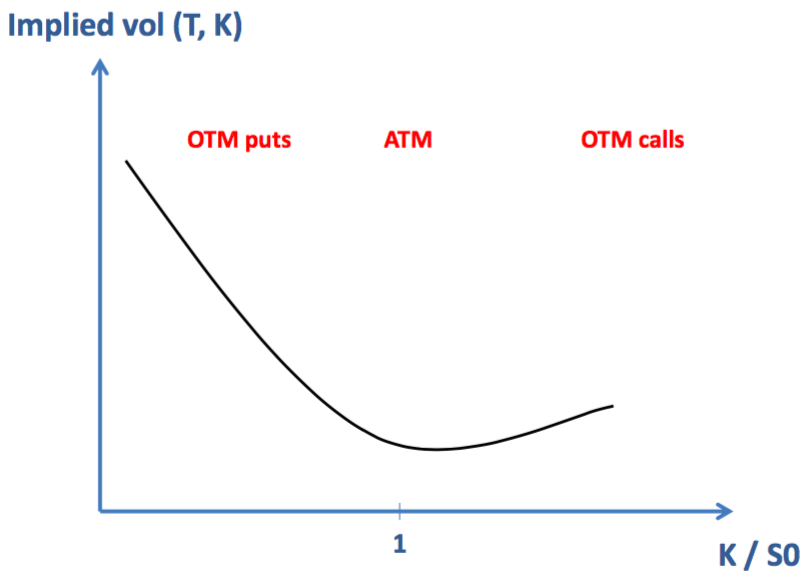
\includegraphics[width=0.7 \linewidth]{IVslice}
\caption{Implied volatility (IV) slice.}
\end{figure}

\paragraph{Drivers/causes for the volatility skew}
\begin{itemize}
\item \emph{Crash-o-phobia/fear of downward price jumps:} Behavioral explanation based on people having developed such a fear after the crash of 1987. Consequently, low-strike put options were suddendly higher priced than high-strike call options, thus increasing the IV for lower strikes.
\item \emph{Leverage effect:} This arises from the negative correlation between stock prices and volatility. Indeed, if the stock price decreases, the debt-to-equity ratio increases and therefore the risk of the firm increases, which translates into higher volatility.
\end{itemize}
\textit{Remark:} In theory, the IVS should be flat in the BS model. The existence of the skew reflects the inability of the normal distribution to capture the movements of returns. Thus, the risk-neutral distribution of returns should be fatter-tailed and in line with the RND inferred from the Breeden-Litzenberger formula.

\paragraph{Requirement for the IVS}
\begin{itemize}
\item A complete IVS is necessary for trading derivatives in general because traders need to quote OTC options with strikes/maturities not quoted on the exchanges.
\item Furthermore, accurate valuation and hedging of structured products strongly depends on the IVS (since structured products can often be decomposed into several basic financial derivatives).
\end{itemize}

\paragraph{NA conditions on call prices}
\begin{align*}
-e^{r_{t,T} (T-t)} \leq \frac{\partial C}{\partial K} \leq &0 \\
&0 \leq \frac{\partial^2 C}{\partial K^2} \\
\frac{\partial C}{\partial T} \leq &0 \\
\left( e^{-q_{t,T}(T-t)} S_t - e^{-r_{t,T}(T-t)} K \right)^+ \leq &C \leq e^{q_{t,T}(T-t)} S_t
\end{align*}
\textit{Remarks:}
\begin{itemize}
\item First condition: Since the call with lower strike has a higher payoff in all future states, it must have a greater value. Thus, the call price $C$ has to be a decreasing function of the strike $K$. \\
Derivation of the first condition: Use the fact that $\partial P/\partial K \geq 0$ (for a similar reasoning) and differentiate the put-call parity once.
\item Second condition: In other words, this condition simply forces the risk-neutral density of the index to be non-negative and/or that all butterfly spreads have non-negative value. \\
Derivation of the second condition: Write the second derivative as infinitesimal butterfly spread.
\item Third condition: All calendar spreads need to have positive value.
\item Fourth condition: The payoff of a call is always non-negative and since the holder of a call is not obligated to buy the underlying at maturity as opposed to the holder of a forward, the price of an equivalent forward functions as another lower bound for any calls.
\end{itemize}

\subsection{Relationship between IV surface and LV surface}

The \emph{IV surface} is a function $\sigma_{\text{imp}} = \sigma_{\text{imp}}(K,T)$ of strike $K$ and maturity $T$.

The \emph{LV surface} is a function $\sigma = \sigma(S,T-t)$ of the stock price value $S$ and time-to-maturity $T-t$.

\paragraph{Flat IVS}
\begin{align*}
\sigma(K,T) = \sigma_{\text{imp}}
\end{align*}
I.e. the local volatility $\sigma$ at future time $T$ and spot value $S_T=K$ is equal to the IV.

\paragraph{Time dependent IVS}
If $\sigma_{\text{imp}} = \sigma_{\text{imp}}(T)$, then local variances $\sigma$ are the derivateve of total implied variances $T \sigma_{\text{imp}}^2$. Hence the implied variance $\sigma_{\text{imp}}$ for maturity $T$ is the average of the local variance from today $t=0$ to this maturity $T$. I.e.
\begin{align*}
\sigma^2(T) &= (T \sigma_{\text{imp}}^2)'(T) \\
\sigma_{\text{imp}}^2(T) &= \frac{1}{T} \int_0^T \sigma^2(t) dt
\end{align*}
Hence in a time-dependent LV model, the option prices can be valued by plugging in the average LV up to time $T$ into the BS formula.

\paragraph{Strike and time dependent IVS}
As soon as the IV surface depends on the strike, the LV function depends on stock price and time (even when the IVs do not depend on maturity. Here, no more simple formulas are available in general.

\subsection{Volatility and variance swaps}

\paragraph{Trading volatility}
\begin{itemize}
\item Hedging volatility risk of any financial asset or derivative requires \emph{variance swaps} that enable direct trading on volatility.
\item Volatility and variance swaps provide a direct exposure to variance without the need to delta-hedge the underlying stock exposure.
\item In other words, they provide a protection against market crashes, i.e. they diversify equity risk.
\end{itemize}

\paragraph{VIX}
\begin{itemize}
\item The \emph{Volatility Index (VIX)} represents the expected future realized volatility of the S\&P500 index returns over the text month. \\
It became since its inception in 1993 a \emph{standard measure of volatility risk} for investors in the US market.
\item There is strong negative correlation between the VIX and the S\&P500. Thus, the VIX is also reffered as the \emph{market's fear gauge}.
\item The VIX seems to be mean reverting with sharp upward moves and more regular decreasing patterns.
\end{itemize}

\paragraph{Variance swap}
The holder of a variance swap over $[0,T]$ receives the realized variance and pays the fixed leg $K$ of the swap at maturity $T$. The payoff at $T$ is as follows:
\begin{align*}
H_T^\text{VS} = M(RV_{0,T}^2(N) - K)
\end{align*}
where $M$ denotes the notional in units of variance, $RV^2$ is the realized variance, $N$ the number of trading days and $K$ the strike of the swap.

\textit{Remarks:}
\begin{itemize}
\item The strike $K$ is quoted on the market and fixed when trading this contract.
\item At settlement, the holder or buyer has to pay its counterparty depending on the sign of the payoff.
\item These contracts are cash settled.
\item Without jumps (or only small jumps) the squared VIX is equal to (or close to) the variance swap rate (at least over the next 30 days).
\end{itemize}
For a variance swap, the fair value of the strike $K$ is the risk-neutral expected future realized variance:
\begin{align*}
K = \mathbb{E}_\mathbb{Q}[RV_{0,T}^2(N)]
\end{align*}

\paragraph{Volatility swap}
A volatility swap allows investors to trade the future realized volatility against a fixed strike. The payoff is as follows:
\begin{align*}
H_T^\text{VolS} = M(RV_{0,T}(N) - K)
\end{align*}
where $M$ denotes the notional in units of volatility, $RV$ is the realized volatility, $N$ the number of trading days and $K$ the strike of the swap.

An upper bound on the strike $K$ of a volatility swap is given by
\begin{align*}
K = \mathbb{E}_\mathbb{Q}[RV_{0,T}(N)] \leq \sqrt{\mathbb{E}_\mathbb{Q}[RV_{0,T}^2(N)]}
\end{align*}
Remark:
\begin{itemize}
\item Even though investors like to think in terms of volatility (and not variance), volatility swaps are much less popular than variance swaps because they are much harder to hedge.
\end{itemize}

\paragraph{Replication of a RV\textsuperscript{2} swap}
The realized variance $RV_{0,T}^2(N)$ can be written in the following way:
\begin{align*}
& RV_{0,T}^2(N) = \underbrace{\sum_{i=1}^N 2U \left( \frac{1}{F_{i-1}} - \frac{1}{F_0} \right) (F_i - F_{i-1})}_\text{I: dynamic position in futures} \\
& \quad + \underbrace{\int_{F_0}^\infty \frac{2 U}{E^2} (F_N - E)^+ dE + \int_0^{F_0} \frac{2 U}{E^2} (E - F_N)^+ dE}_\text{II: static position in European options} \\
& \quad + \underbrace{\sum_{i=1}^N \mathcal{O}(R_i^3)}_\text{III: error term}
\end{align*}
where $F_i$ denote the futures at time $t$ with identical maturity $T$, $U = \frac{252}{N}$ and $F_i := F_{t_i}$.

\textit{Remarks:}
\begin{itemize}
\item Term \emph{I} is a \emph{dynamic position in futures with maturity $T$}. At each time $t_{i-1} (i >1)$, one should hold $2U \left( \frac{1}{F_{i-1}} - \frac{1}{F_0} \right)$ futures contracts (with price $F_{i-1}$ at time $t_{i-1}$).
\item Term \emph{II} is a \emph{static position in European options}. AT time $t_0 = 0$, one should hold $\frac{2U dE}{E^2}$ European call options at all strikes $E > F_0$ where $dE$ is the increment between strikes available in practice. One should also hold $2U \left( \frac{1}{F_{i-1}} - \frac{1}{F_0} \right)$ European put options at all strikes $E < F_0$. \\
The construction of this static part theoretically relies on the Breeden-Litzenberger static hedging formula of European style contingent claims.
\end{itemize}

\paragraph{Fair strike of a variance swap}
\begin{align*}
K &= \int_{F_0}^\infty \frac{2 U}{E^2} e^{r (T-t_0} C(t_0,F_0,E,T) dE \\
& \quad + \int_0^{F_0} \frac{2 U}{E^2} e^{r (T-t_0} C(t_0,F_0,E,T) dE
\end{align*}
To compute $K$, it is standard practice to write the integral as a discrete sum over available strikes.

Drawbacks:
\begin{itemize}
\item The assumed \emph{continuum of strikes} is in practice not available. Especially when the market dries up and deep OTM options are not traded anymore, this hedge does not work well in practice.
\item The hedge \emph{understimates the realized variance}. In other words, it neglects skewness and kurtosis effects.
\end{itemize}

\columnbreak

\section{Extensions of the Black-Scholes Model}

\paragraph{Advantages of the BS model}
\begin{itemize}
\item Options can be easily replicated by trading the underlying stock and a risk-free bond.
\item Option prices are given in closed-form.
\end{itemize}

\paragraph{Shortcomings of the BS model}
\begin{itemize}
\item Since the BS model assumes constant volatility, it is not consistent with the IVS observed in the equity markets.
\end{itemize}

\subsection{Local Volatility Models (LV Models)}

\paragraph{Definition}
\begin{itemize}
\item LV models are one-factor stochastic volatility models where the volatility depends on the stochastic evolvement of the stock price $S_t$ and time $t$, i.e. $\sigma = \sigma(S_t,t)$. \\
In other words, volatility $(\sigma(S_t,t)_{t \geq 0}$ is stochastic but at time $t$ entirely determined by the price $S_t$, i.e. the volatility is indirectly stochastic.
\item Consequently, the market is still \emph{complete} and thus all contingent claims can be perfectly hedged.
\end{itemize}

\subsubsection{Local volatility as a special case of stochastic volatility}

\paragraph{Dynamics under the risk-neutral measure $\mathbb{Q}$}
Most of the one-factor continuous dynamics under $\mathbb{Q}$ can be summarized by:
\begin{align*}
\frac{dS_t}{S_t} &= r_t dt + \sigma (S_t,t) dW_t \\
d \sigma(S_t,t) &= \mu_\sigma (S_t,t,\sigma) dt + \nu_\sigma (S_t,t,\sigma) dZ_t
\end{align*}
where $W$ and $Z$ are $\mathbb{Q}$-Brownian motions possibly correlated via $d[W,Z]_t = \rho dt$.

\paragraph{Dynamics under the historical measure $\mathbb{P}$}
\begin{align*}
\frac{dS_t}{S_t} &= \mu(S_t,t) dt + \sigma (S_t,t) d \tilde W_t
\end{align*}
where $\tilde W$ is a $\mathbb{P}$-Brownian motion.

\paragraph{Example: CEV model}

The \emph{Constant Elasticitiy of Variance (CEV)} model was developed by Cox and Ross (1976). The underlying has the following dynamics:
\begin{align*}
dS_t &= \mu (S_t,t) dt + \sigma S_t^\beta dZ_t & \beta, \sigma \geq 0
\end{align*}
Most often, the following simple $\mathbb{Q}$-dynamics is considered:
\begin{align*}
dS_t &= r S_t dt + \sigma S_t^\beta dW_t
\end{align*}
\textit{Remarks:}
\begin{itemize}
\item $\beta = 1$ corresponds to the BS model
\item $\beta = 0$ corresponds to the Bachelier model, which assigns a normal distribution to the stock price (consequently, the stock price can become negative in this model)
\item When $0 < \beta < 1$, the model is able to reproduce the \emph{leverage effect}, i.e. the volatility increases when the stock price goes down, which is observed empirically.
\item While the model is able to reproduce a leverage effect and skewed implied volatilities, it is not able to fit an arbitrary smile of implied volatility since it is parametric (with two parameters). Non-parametric models are able to produce much better fits.
\end{itemize}

\paragraph{LV models and IV smile}
In a LV framework the static properties of IVs (as a function of strike and maturity) determine the way the IV smile will behave dynamically in the future.

\subsubsection{Option pricing in LV models}

\paragraph{Martingale pricing in LV models}
The fair value $V_t$ of a European style contingent claim with payoff $h(S_T)$ is given by
\begin{align*}
V_t &= \mathbb{E}_\mathbb{Q} \left[ \left. e^{-\int_t^T r_s ds} h(S_T) \right| \mathcal{F}_t \right]
\end{align*}
\textit{Remarks:}
\begin{itemize}
\item $r_s$ is the deterministic risk-free rate.
\item Because $\sigma$ soley depends on $S$ and $t$ and not on new sources of randomness, the BS PDE is still satisfied by $V(t,S)$ in the LV model.
\end{itemize}

\paragraph{Dupire Formula}
\begin{align*}
\frac{\partial C}{\partial T} &= \frac{1}{2} \sigma (K,T)^2 K^2 \frac{\partial^2 C}{\partial K^2} - q_T C - K(r_T - q_T) \frac{\partial C}{\partial K}
\end{align*}
which is equivalent to
\begin{align*}
\sigma (K,T)^2 &= \frac{\frac{\partial C}{\partial T} + q_T C + (r_T - q_T) K \frac{\partial C}{\partial K}}{\frac{1}{2} K^2 \frac{\partial^2 C}{\partial K^2}}
\end{align*}
\textit{Remarks:}
\begin{itemize}
\item $C = C(t,S,T,K)$
\item $r_T$ is the instantaneous deterministic interest rate, which is related to $r_{0,T}$ by the relation $r_{0,T} = \frac{1}{T} \int_0^T r_s ds$.
\item This equation holds for $S = S_0$ and $t = t_0$ fixed. Hence it provides no information about the dynamics of the model.
\item It determines how the implied volatility smile today has to behave in the direction of strike and maturity.
\end{itemize}

\paragraph{Backward Kolmogorov equation}
\begin{align*}
\frac{\partial C}{\partial t} + (r-q) S \frac{\partial C}{\partial S} + \frac{1}{2} \sigma (S,t)^2 S^2 \frac{\partial^2 C}{\partial S^2} = r C
\end{align*}
\textit{Remarks:}
\begin{itemize}
\item $C = C(t,S,T,K)$, $T$ and $K$ are fixed and the equation is subject to: \\
\emph{Terminal condition:} $C_T(K,T) = (S-K)^+$.
\item This PDE determines the dynamic evolution of call prices or equivalently implied volatilities.
\item This PDE actually holds for arbitrary European style contingent claims with payoff $V(S_T,T) = H(S_T)$.
\item This PDE is written in terms of $(t,S)$, thus the variables $T,K$ are considered to be fixed.
\item Once the local volatility function $\sigma$ has been estimated, this PDE can be solved numerically IOT determine prices.
\item It is called \emph{backward} since it shows how the price $C$ propagates backward in time from its value at maturity $C(T,S_T) = h(S_T)$ to its value today $V(0,S_0)$.
\item It is not possible to solve this equation for an arbitrary LV function $\sigma(S,t)$. \\
Thus, numerical methods are necessary to approximate prices of options. Most common are Monte-Carlo, Tree and Finite difference methods.
\end{itemize}

\paragraph{Fokker-Planck equation} (Also known as the \emph{forward Kolmogorov equation})
\begin{align*}
\frac{\partial f}{\partial T}(S,T) &= -\frac{\partial}{\partial S} \left( (r_T - q_T) S f(S,T) \right) \\
& \qquad + \frac{1}{2} \frac{\partial^2}{\partial S^2} \left( \sigma(S,T)^2 S^2 f(S,T) \right)
\end{align*}
\textit{Remarks:}
\begin{itemize}
\item The Fokker-Planck equation describes the evolution of the \emph{risk-neutral probability density function} $f_T^S = f(S,T)$ of the stochastic process given by the risk-neutral dynamics of the LV model up to time/maturity $T$.
\item The equation is called \emph{forward} since the initial probability density of the stock price at $t=0$ is known, i.e. it is Dirac delta function center at $S = S_0$. \\
\emph{Initial condition: } $f(S=S_0,T=0) = \delta_{S_0}(S)$ \\
As time evolves, this Dirac mass evolves according to the Fokker-Planck equation.
\end{itemize}

\paragraph{Local volatility as a function of the implied volatility}
From the \emph{Dupire formula}, the following expression can be derived.
\begin{align*}
& \sigma (K,T)^2 = \\
& \frac{\sigma_{\text{imp}}^2 + 2 \sigma_{\text{imp}} T \left( \frac{\partial \sigma_{\text{imp}}}{\sigma_{\text{imp}} T} + (r_T - q_T) K \frac{\partial \sigma_{\text{imp}}}{\partial K} \right)}{\text{denominator}} \\ \\
& \text{denominator} = \left( 1 - \frac{K}{\sigma_{\text{imp}}} \frac{\partial \sigma_{\text{imp}}}{\partial K} \right)^2 \\
& + K \sigma_{\text{imp}} T \left( \frac{\partial \sigma_{\text{imp}}}{\partial K} - \frac{1}{4} K \sigma_{\text{imp}} T \left( \frac{\partial \sigma_{\text{imp}}}{\partial K} \right)^2 + K \frac{\partial^2 \sigma_{\text{imp}}}{\partial K^2} \right)
\end{align*}

\subsubsection{Debate of LV models}

\paragraph{Advantages/useful features}
\begin{itemize}
\item It is a stochastic volatility model where volatility depends on the random realization of the stock price.
\item \emph{Many useful properties of the BS model remain valid}, e.g. all European style contingent claims are hedgable and the EMM is unique (i.e. the marekt is complete). This is due to the fact that the local volatility process is merely a function of the stock price process (and time).
\item The LV function is given by Dupire's formula. Hence, for a given smooth IV surface, there exists a unique LV function that allows replicating all option prices.
\item \emph{Pricing derivatives is fast} since there is only one stochastic factor (i.e. the stock price $S$), i.e. when using the backward Kolmogorov equation and finite difference/elements technique.
\end{itemize}

\paragraph{Disadvantages/criticism}
\begin{itemize}
\item \emph{The LV model is making predictions that are consistently wrong over time.} \\
In other words, although a LV model can price European options very accurately, the dynamics that the stock price process follows are inaccurate. \\
Hence hedging with LV models can give poor results. There is no LV model $\sigma(S,t)$ capable of reproducing the dynamics of the smile, and actually the dynamics of the smile of volatility implied by LV models seem to be even worse than those of the simple BS model.
\item In the LV framework, if the stock prices increases by $\Delta S_0 > 0$, then the IV surface will move to the left. In fact, this is opposite to the typical behavior observed in markets. \emph{The LV model therefore introduces wrong dynamics for the IVS.}
\end{itemize}
Having said this, it turns out that these criticism are only valid when the LV function can be written as $\sigma(S,t)$ and not as a function of the initial spot price as well, i.e. $\sigma = \sigma(S,t,S_0)$. In these models, the smile movements predicted when the spot moves can be in line with what is observed on actual markets.

\subsection{Stochastic Volatility: The Heston Model}

\subsubsection{General stochastic volatility models}

\paragraph{Initial remarks}
\begin{itemize}
\item Here, two-factor stochastic volatility models are considered, i.e. the volatility is modelled itself as a stochastic process, introducing some additional randomness.
\item Stochastic volatility models are not needed to replicate the prices of European options observed on a given date, but to model accurately the \emph{dynamics of volatility}.
\item Hence, stochastic volatility models are applied to \emph{derivates sensitive to future volatility levels}, e.g. Variance swaps (OTC), VIX futures and VIX options.
\end{itemize}

\paragraph{Dynamics of general two-factor stochastic volatility models}
\begin{align*}
dS_t &= \mu_S (S_t,V_t,t) dt + \sigma_S (S_t,V_t,t) dZ_t \\
dV_t &= \mu_V (S_t,V_t,t) dt + \sigma_V (S_t,V_t,t) dW_t \\
V_t &= g(\sigma_S) \\
\mathbb{E} [dW_t dZ_t] &= \rho dt
\end{align*}
\textit{Remarks:}
\begin{itemize}
\item $S_t$ is the stock price and $V_t$ the volatility.
\item The process $\sigma_S$ is the instantaneous volatility of the returns process.
\item The variance of the underlying process is now itself a stochastic process driven by a Brownian motion $W_t$ which is correlated with $Z_t$, with instantaneous correlation coefficient $\rho$.
\end{itemize}

\paragraph{Assumptions}
\begin{itemize}
\item The correlation between the stock movements and those of its volatility are assumed constant. In practice, the correlation is often considered time-varying.
\item The general model above has only one random factor for the volatility while econometric studies have shown that the IVS is generated by several factors.
\end{itemize}

\paragraph{Completeness of the market}
\begin{itemize}
\item The market is now \emph{incomplete} since there are at least two sources of randomness.
\item \emph{Perfect dynamic replication} of an option by trading the stock $S$ and the risk-free bond $B$ is not possible anymore since the random term $W$ in the volatility is not tradable if only these two assets are used for a replicating portfolio, i.e. $W$ cannot be hedged using just bonds and stocks.
\item Consequently, the martingale measure $\mathbb{Q}$ is no more unique and there is now a whole range of arbitrage-free option prices. \\
Hence \emph{additional assumptions} need to be made while different choices of martingale measures will lead to different prices.
\item IOT hedge all risks, another option can be used as hedging instrument, e.g. high vega products.
\end{itemize}

\subsubsection{Dynamics of the Heston Model}

\paragraph{Dynamics under the historical measure $\mathbb{P}$}
\begin{align*}
\frac{dS_t}{S_t} &= \mu dt + \sqrt{V_t} dZ_t \\
dV_t &= \kappa (\theta - V_t) dt + \eta \sqrt{V_t} dW_t \quad , \quad 2 \kappa \theta > \eta^2 \\
d[Z,W]_t &= \rho dt
\end{align*}
\textit{Remarks:}
\begin{itemize}
\item The variance follows a Cox-Ingersoll-Ross (CIR) process.
\item Due to the \emph{Feller condition} $2 \kappa \theta > \eta^2$, the variance cannot go negative.
\item Furthermore, the variance is \emph{mean-reverting}, with: \\
$\kappa>0$ the \emph{speed of mean-reversion}, \\
$\theta>0$ the \emph{level of mean reversion}.
\item Intuitively, this means that when the volatility moves away from its level of mean reversion, the drift $\kappa (\theta - V_t) dt$ will pull it back towards $\theta$.
\item The parameter $\eta>0$ denotes the volatility of volatility, also called \emph{volvol}.
\item The so-called \emph{long-term mean of volatility} is equal to the level of mean reversion, i.e.
\begin{align*}
\lim \limits_{t \rightarrow \infty} \mathbb{E}[V_t] = \theta
\end{align*}
\item \emph{Leverage effect:} The correlation coefficient $\rho$ is usually found to be strongly negative, i.e. negative shocks in returns and positive shocks in volatility usually happen simultaneously. This can be seen as a cause of the volatility skew.
\end{itemize}
Due to the correlation between the two BMs $Z$ and $W$, the BM $Z$ can be equivalently rewritten as $Z = \rho W + \sqrt{1-\rho^2} W^\bot$, where $W^\bot$ is a $\mathbb{P}$-BM a.s. Thus the stock dynamics can be rewritten as
\begin{align*}
\frac{dS_t}{S_t} &= \mu dt + \sqrt{V_t} \left( \rho dW_t + \sqrt{1-\rho^2} dW_t^\bot \right)
\end{align*}

\paragraph{Dynamics under the risk-neutral measure $\mathbb{Q}$}
\begin{align*}
\frac{dS_t}{S_t} &= r dt + \sqrt{V_t} d \tilde Z_t \\
dV_t &= \kappa \left(\theta - V_t + \frac{\eta}{\kappa} \sqrt{V_t} \alpha_t^1 \right) dt + \eta \sqrt{V_t} d \tilde W_t
\end{align*}
\textit{Remarks:}
\begin{itemize}
\item The adapted process $\alpha_t^1$ has to be (arbitrarily) determined.
\item The choice of Heston $\alpha_t^1 := \lambda \sqrt{V_t}$ ensures that the technical conditions are satisfied and that the process $V_t$ remains a CIR process under $\mathbb{Q}$ (which is necessary to compute closed-form option prices).
\end{itemize}
 Then the dynamics of the volatility becomes
\begin{align*}
dV_t &= \kappa^\ast (\theta^\ast - V_t) dt + \eta \sqrt{V_t} d \tilde W_t \\
\kappa^\ast &= \kappa - \lambda \eta \quad , \quad \theta^\ast = \frac{\kappa}{\kappa^\ast} \theta
\end{align*}
and to ensure that $\mathbb{Q}$ is an EMM, it needs to hold that
\begin{align*}
\alpha_t^2 &= \frac{1}{\sqrt{1-\rho^2}} \left( \frac{\mu-r}{\sqrt{V_t}} - \rho \lambda \sqrt{V_t} \right)
\end{align*}

\paragraph{Feller Condition}
If $2 \kappa \theta > \eta^2$, then $V_t > 0, \forall t \geq 0$, $\mathbb{P}$-a.s., i.e. the variance will never reach zero $\mathbb{P}$-a.s. \\
\textit{Remarks:}
\begin{itemize}
\item Intuitively, this conditions bounds the amplitude $\eta$ (volvol) of the shocks in the variance.
\item If $\eta$ (volvol) is too high, then the Brownian shocks may be too big and the process may become negative.
\item If $\kappa$ (speed of mean reversion) is too low, then the process does not revert quickly enough to its level reversion, meaning that $V_t$ may get quite far from $\theta >0$, and may reach zero.
\item If $\theta$ (level of mean reversion) is too low, then the process reverts to a very low level, which inreases the possibility of $V_t$ reaching zero.
\end{itemize}

\subsubsection{Heston PDE}

\paragraph{Replicating portfolio for an option in the Heston model}
Here three different assets are required for the replicating portfolio, in particular one new asset exposed to the volatility random term $dW_t$. One solution is to consider another option.

Here it is assumed that we want to price an option with price $C_t^1$ at time $t$. Hence a self-financing portfolio is considered where we have bought one unit of this option $C_t^1$, sold an amount $a_t$ of another option with price $C_t^2$ and sold an amount $b_t$ of shares at time $t$.
\begin{align*}
\pi_t &= C^1(t,S_t,V_t) - a_t C^2(t,S_t,V_) - b_t S_t \\
d \pi_t &= r \phi_t dt = r(C_t^1 - a_t C_t^2 - b_t S_t) dt
\end{align*}
By the \emph{self-financing property} (and Itô's formula):
\begin{align*}
d\pi = dC^1 - a_t dC^2 - b_t dS_t
\end{align*}
and by \emph{absence of arbitrage}:
\begin{align*}
d \pi_t &= r \phi_t dt = r(C_t^1 - a_t C_t^2 - b_t S_t) dt.
\end{align*}
The \emph{weights in the replicating portfolio} can be computed as
\begin{align*}
a_t &= \frac{\partial_V C^1}{\partial_V C^2} & b_t &= \partial_S C^1 - \frac{\partial_V C^1}{\partial_V C^2} \partial_S C^2
\end{align*}

\paragraph{Infinitesimal generator for a stochastic process}
Let $X: [0,\infty) \times \Omega \rightarrow \mathbb{R}^n$ be defined on a probability space $(\Omega, \mathcal{F}, \mathbb{P})$ satisfying the following SDE:
\begin{align*}
dX_t = b(X_t) dt + \Sigma (X_t) dB_t
\end{align*}
where $B$ is an $m$-dimensional Brownian motion (with independent components), $b: \mathbb{R}^n \rightarrow \mathbb{R}^n$ is the drift function and $\Sigma : \mathbb{R}^n \rightarrow \mathbb{R}^{n \times m}$ is the diffusion function. For a point $x \in \mathbb{R}^n$, let us denote $\mathbb{P}^x$ the law of $X$ given the initial point $X_0 = x$ and let us denote $\mathbb{E}^x$ the expectation w.r.t. $\mathbb{P}^x$. The infinitesimal generator of $X$ is the operator $\mathcal{A}$ defined, for a suitable class of function $f: \mathbb{R}^n \rightarrow \mathbb{R}$, as:
\begin{align*}
\mathcal{A} f(x) = \lim\limits_{t \rightarrow 0} \frac{\mathbb{E}^x[f(X_t)] - f(X_0)}{t}
\end{align*}
It can be shown that $\mathcal{A}$ is the operator defined by the property that $\{ f(X_t) - \int_0^t \mathcal{A} f(X_s) ds, t \geq 0 \}$ is a martingale for all $f$ in the domain of the generator. As a consequence:
\begin{align*}
\mathcal{A} f(x) &= \sum_{i=1}^n b_i(x) \frac{\partial f}{\partial x_i}(x) \\
& \quad + \frac{1}{2} \sum_{i,j=1}^n (\Sigma(x) \Sigma(x)^T)_{i,j} \frac{\partial^2 f}{\partial x_i \partial x_j}(x)
\end{align*}

\paragraph{Infinitesmial generator of the Heston model}
The infinitesmial generator of the Heston model $\{ (S_t,V_t), t \geq 0 \}$ under $\mathbb{P}$ and under $\mathbb{Q}$, respectively, is:
\begin{align*}
\mathcal{A}_\text{Heston}^\mathbb{P} &= \mu S \frac{\partial}{\partial S} + \frac{1}{2} V S^2 \frac{\partial^2}{\partial S^2} - \kappa (V-\theta) \frac{\partial}{\partial V^2} \\
& \quad + \frac{1}{2} \eta^2 V \frac{\partial^2}{\partial V^2} + \rho \eta V S \frac{\partial^2}{\partial S \partial V} \\
\mathcal{A}_\text{Heston}^\mathbb{Q} &= r S \frac{\partial}{\partial S} + \frac{1}{2} V S^2 \frac{\partial^2}{\partial S^2} + (\kappa(\theta - V) - \lambda V) \frac{\partial}{\partial V} \\
& \quad + \frac{1}{2} \eta^2 V \frac{\partial^2}{\partial V^2} + \rho \eta V S \frac{\partial^2}{\partial S \partial V}
\end{align*}

\paragraph{Market price of volatility risk $\Phi(S_t,V_t,t)$}
In the Heston model, the market price of volatility risk is not specified as a consequence of market incompleteness. Hence one could take any function $\Phi(S_t,V_t,t$ and obtain arbitrage-free prices. \\
Heston assumed that the market price of volatility risk is linear in the instantaneous variance, i.e.
\begin{align*}
\Phi (S_t, V_t,t) = \Phi (V_t) = \lambda V_t
\end{align*}

\paragraph{Risk premium of the option $C$}
The risk premium of the option $C$ is a weighted average of the market price of equity risk ($\mu-r$) and the market price of volatility risk $\Phi(S_t,V_t,t)$.
\begin{align*}
\underbrace{\mu_C - r}\limits_\text{risk premium} = \frac{\sigma_\text{CS}}{\sqrt{V_t}} \underbrace{(\mu-r)}\limits_\text{equity risk} + \frac{\sigma_\text{CV}}{\sqrt{V_t}} \underbrace{\Phi(S_t,V_t,t)}\limits_\text{market price of volatility risk}
\end{align*}

\paragraph{Heston PDE}
Under the historical probability measure $\mathbb{P}$ or under a risk-neutral probability measure $\mathbb{Q}$, respectively, the Heston PDE can be written as:
\begin{align*}
\partial_V C \Phi(S,V,t) &= -r C + \partial_t C + \mathcal{A}_\text{Heston}^\mathbb{P} C - (\mu - r) S \partial_S C \\
0 &=-r C + \partial_t C + \mathcal{A}_\text{Heston}^\mathbb{Q} C
\end{align*}
Remark: The Heston PDE (under the risk-neutral measure $\mathbb{Q}$) actualy holds irrespective of the stochastic process chosen to model volatility. Only the infinitesimal generator $\mathcal{A}^\mathbb{Q}$ has to be adjusted accordingly.

\subsubsection{Option prices in the Heston model}

\paragraph{Solution of the Heston PDE}
\begin{enumerate}
\item Change of variables
\item Fourier transformation
\item Insert Ansatz for the Fundamental solution back into Fourier transformed PDE
\item Solve Ricatti equation
\end{enumerate}

\paragraph{Option price in the Heston model}
\begin{align*}
C(k,\tau) &= \kappa \theta \left( r_1 \tau - \frac{2}{\eta^2} \log \left( \frac{1 - g e^{d \tau}}{1 - g} \right) \right) \\
\tau &= T-t \quad , \quad g = \frac{r_1}{r_2}
\end{align*}
Due to singularities triggered by the complex logarithm in the Heston model, the call price function can be adjusted by a rotation count algorithm as follows:
\begin{align*}
C^\text{adj}(k,\tau) &= \kappa \theta \left( r_2 \tau - \frac{2}{\eta^2} \log \left( \frac{1 - g e^{d \tau}}{1 - g} e^{-d \tau} \right) \right)
\end{align*}

\subsubsection{Debate of the Heston model}

\paragraph{Performance/advantages}
The Heston model is widely used in practice for the following advantages/useful features:
\begin{itemize}
\item It exhibits \emph{mean reversion of volatility}.
\item It is relatively simple to understand and implement.
\item It allows to accurately represent the IVS and better captures the dynamics of the IVS than LV models.
\end{itemize}

\paragraph{Disadvantages/criticism/pitfalls:}
\begin{itemize}
\item The \emph{volatility applied in the Heston model is not observable}, hence its initial value $V_0$ required to price options cannot be read from the market. \\
Instead, this value has to be calibrated together with the other parameters IOT fit option prices.
\item The implied skew is often too flat for short maturities, while for longer maturities the model performs much better. In other words, \emph{the Heston model is not capable of generating high enough implied volatilites for short maturities}. \\
This means that the $\mathbb{Q}$-density of the Heston returns has too little mass in the left tail (negative returns). \\
I.e. it features \emph{a skew which is not steep enough for short maturities}.
\item There is a trade-off between enforcing the calibrated parameters to fulfil the \emph{Feller condition} and making the parameters best fit the observed option prices on the market (\emph{fit of option prices}).
\end{itemize}

\paragraph{Alternative modelling approaches}
\begin{itemize}
\item volatility as an Ornstein-Uhlenbeck process
\item volatility as a non-mean-reverting process lognormally distributed
\item volatility as the exponential of a mean-reverting Ornstein-Uhlenbeck process
\end{itemize}

\subsubsection{Calibration of the Heston model}

The most widely used calibration method is the \emph{least-square estimation}, which consists in minimizing the errors between the prices predicted by the model and the market prices. The minimization function and its output parameter are
\begin{align*}
& \min\limits_{\Theta} \left\lbrace LS(\Theta) := \sum_{i=1}^N \hat \epsilon_i (K_i,T_i) \right\rbrace \\
& \quad \hat \Theta = \arg \min_\Theta LS(\Theta)
\end{align*}
where $\epsilon_i (K_i,T_i)$ is a function of the market price of the option $C_i^\text{obs}$ with strike $K_i$ and maturity $T_i$ and of the model price $C_i(K_i,T_i,\Theta$.

The function $\epsilon$ represents an appropriate distance and the variable $\Theta$ represents the vector of parameters that we wish to estimate.

For $\epsilon$, one could e.g. take the \emph{absolute error} or the \emph{Euclidean distance}:
\begin{align*}
\hat \epsilon_i(K_i,T_i) &= \left| C_i^\text{obs} - C_i(K_i,T_i,\Theta) \right| \\
\hat \epsilon_i(K_i,T_i) &= \left( C_i^\text{obs} - C_i(K_i,T_i,\Theta) \right)^2
\end{align*}

However, these choices for $\epsilon$ give more weight to expensive options (i.e. ITM option). To correct for this, one can instead minimize \emph{relative distances} instead of absolute distances:
\begin{align*}
\hat \epsilon_i (K_i,T_i) = \frac{|C_i^\text{obs} - C_i(K_i,T_i,\Theta|}{C_i^\text{obs}}
\end{align*}
However, this choice favours cheaper options, and in particular short-term options. One can hence add weights IOT emphasize certain options:
\begin{align*}
\hat \epsilon_i(K_i,T_i) = \omega_i (\sigma_\text{imp,i}^\text{obs} - \sigma_\text{imp,i}(K_i,T_i,\Theta))^2
\end{align*}

IOT deal with the issue of local minima (IOT ensure that a global minimum is found), one can either take different optimization algorithms (e.g. the Differential Evoluation algorithm) or \emph{regularize} the given problem by adding a term to the objective function IOT make it \emph{convex}:
\begin{align*}
LS^\text{reg} (\Theta) = \sum_{i=1}^N \omega_i (\sigma_\text{imp,i}^\text{obs} - \sigma_\text{imp,i}(K_i,T_i,\Theta))^2 + \alpha p(\Theta)
\end{align*}
where $\alpha$ is called the regularisation parameter and $p$ the penalty function.

\subsection{Jump Models: Lévy processes}

\subsubsection{Merton's Jump Diffusion Model}

\paragraph{Stock price under the historical measure $\mathbb{P}$}
\begin{align*}
S_t &= S_0 \exp (L_t) \\
L_t &= \underbrace{\mu t + \sigma W_t}\limits_\text{continuous part} + \underbrace{\sum_{k=1}^{N_t} Y_k}\limits_\text{jump part}
\end{align*}
\textit{Remarks:}
\begin{itemize}
\item $N_t$ is a Poisson process (i.e. counting process)
\item $(Y_k)_{k \geq 1}$ is a collection of i.i.d. normally distributed RVs \\
i.e. $Y_k \sim \mathcal{N}(\mu_Y,\sigma_Y^2$ with normal density
\begin{align*}
f_Y(y) = \frac{1}{\sqrt{2 \pi} \sigma_Y} \exp \left[ - \frac{(y - \mu_Y)^2}{2 \sigma_Y^2} \right]
\end{align*}
\item Thus, $\left( \sum_{k=1}^{N_t} Y_k \right)_{t \geq 0}$ is a compound Poisson process.
\end{itemize}

\paragraph{Jump process}
The jump process $(J_s)_{s \geq 0}$ is defined as
\begin{align*}
J_s &:= L_s - L_{s^-} = \sum_{i=1}^{N_s} Y_i - \sum_{i=1}^{N_{s^-}} Y_i \\
J_{\tau_k} &= \sum_{i=1}^{N_{\tau_k}} Y_i - \sum_{i=1}^{N_{\tau_k^-}} Y_i
\end{align*}
In other words, the jump process only jumps at a countable number of times $\lbrace \tau_k \rbrace_{k \in \mathcal{N}^\ast}$ with normally distributed jump sizes $Y_k$.

\paragraph{Dynamics under the historical measure $\mathbb{P}$}
\begin{align*}
dS_t &= \left( \mu + \frac{\sigma^2}{2} \right) S_{t^-} dt + \sigma S_{t^-} dW_t + S_{t^-} (e^{J_t} -1) dN_t \\
L_t &= L_0 + \mu \int_0^t ds + \sigma \int_0^t dW_s + \sum_{k=1}^{N_t} J_{\tau_k} \\
dL_t &= \mu dt + \sigma dW_t + J_t dN_t
\end{align*}

\paragraph{Incompleteness of the market}
Because of randomness coming from the size and time of jumps, the market is no longer complete.

The risk-neutral process is chosen based on two considerations:
\begin{itemize}
\item The volatility and jump statistics remain unchanged under $\mathbb{Q}$, i.e. only the drift of the original process changes.
\item Under $\mathbb{Q}$, the process $\left( e^{-rt} S_t \right)_{t \geq 0}$ is a martingale.
\end{itemize}

\paragraph{Dynamics under a risk-neutral probability measure $\mathbb{Q}$}
\begin{align*}
\frac{dS_t}{S_{t^-}} &= \alpha dt + \sigma d \tilde W_t + (e^{J_t} - 1) d \tilde N_t \\
\frac{dS_t}{S_{t^-}} &= \left( r - \tilde \lambda \mathbb{E}^\mathbb{Q} \left[ e^{Y_1} - 1 \right] \right) dt + \sigma d \tilde W_t + (e^{J_t} - 1) d \tilde N_t
\end{align*}
\textit{Remarks:}
\begin{itemize}
\item $\alpha = r - \tilde \lambda \mathbb{E}^\mathbb{Q} \left[ e^{Y_1} - 1 \right]$ according to the Martingale condition
\item $\tilde N$ either jups at $t$ with probability $\mathbb{Q}_t(\tilde N_t - \tilde N_{t^-} = 1) = \tilde \lambda dt$ or it does not jump.
\end{itemize}

\paragraph{Stock price under a risk-neutral probability measure $\mathbb{Q}$}
\begin{align*}
S_T &= S_t \exp \left( \left( \mu^\mathbb{Q} - \frac{1}{2} \sigma^2 \right) (T-t) + \sigma \left( \tilde W_T - \tilde W_t \right) \right. \\
& \qquad + \left. \sum_{k=1}^{\tilde N_T - \tilde N_t} Y_k \right)
\end{align*}
where $\mu^\mathbb{Q} = r - \tilde \lambda \mathbb{E}^\mathbb{Q} \left[ e^{Y_1} - 1 \right]$ the risk-neutral drift.

\paragraph{Call price of a European option}
\begin{align*}
C(t,S_t) = \sum_{n=0}^\infty \frac{e^{\tilde \lambda \tau} (\tilde \lambda \tau)^n}{n!} C_\text{BS}(\tau, \hat S_t(n), \sigma_n)
\end{align*}
\textit{Remarks:}
\begin{itemize}
\item $C_\text{BS}(\tau, \hat S_t(n), \sigma_n)$ is the BS call pricing formula for an option with maturity $\tau$, initial underlying value $\hat S_t(n)$ and volatility $\sigma_n$.
\item $\sigma_n = \sigma + \frac{n \sigma_Y^2}{\tau}$
\item This call price can be derived using the martingale approach: \\
$C(t,S_t) = e^{-r(T-t)} \mathbb{E}^\mathbb{Q} \left[ \left. (S_T - K^+ \right| \mathcal{F}_t \right]$.
\end{itemize}

\paragraph{Hedging in the Merton jump diffusion model}
\begin{itemize}
\item Consider a portfolio $\pi$ composed of one option $C$ and $-\alpha$ units of stocks.
\item Instantaneous change of value of $\pi_t$: \\
$d\pi_t = dC_t - \alpha_t dS_t$.
\item Due to market incompleteness stemming from the jumps, portfolio $\pi$ is not risk-free.
\item Merton's assumption: Jumps ($N_t$) uncorrelated with the market, jump risk diversifiable and thus without any risk premium.
\item Under Merton's assumption: portfolio return has to equal the risk-free rate as return: \\
$\mathbb{E}_t^\mathbb{P} \left[ d\pi_t \right] = r \pi_t dt$
\end{itemize}

\paragraph{PDE for the Merton jump diffusion model}
\begin{align*}
&  \frac{\partial C}{\partial t} + r \frac{\partial C}{\partial S} S_{t^-} + \frac{1}{2} \frac{\partial^2 C}{\partial S^2} \sigma^2 S_{t^-}^2 \\
& + \mathbb{E}_\mathbb{P} \left[ C(t,S_{t^-}, e^{Y_1}) - C(t,S_{t^-} \right] \lambda \\
& - \frac{\partial C}{\partial S} \mathbb{E}_\mathbb{P} \left[e^{Y_1} - 1 \right] S_{t^-} \lambda - r C_{t^-} = 0
\end{align*}
where $\mathbb{E}_\mathbb{P} \left[ e^{Y_1} - 1 \right] = \exp \left( \mu_J + \frac{1}{2} \sigma_J^2 \right) -1$.

It is possible to solve this PDE and obtain the price of a European option as a weighted average of an infinite number of BS prices of options with different volatilities.

\subsubsection{Basics of Lévy processes}

\paragraph{Lévy process}
Let ($\Omega, \mathcal{F}, (\mathcal{F}_t), \mathbb{P})$ be a filtered probability space with satisfies the usual conditions. Let $T \in [0, \infty]$. A càdlàg, adapted, real valued stochastic process $L = (L_t)_{0 \leq t \leq T}$ is called a Lévy process if it satisfies the following conditions:
\begin{itemize}
\item $L_0 = 0$.
\item $L$ has \emph{independent increments}, i.e. $L_t - L_s$ is independ of $\mathcal{F}_s$ for any $0 \leq s < t \leq T$.
\item $L$ has \emph{stationary increments}, i.e. for any $0 \leq s$, $t \leq T$ the distribution of $L_{t+s} - L_t$ does not depend on $t$.
\item $L$ is \emph{stochastically continuous}, i.e. for every $0 \leq t \leq T$ and $\epsilon > 0$, $\lim_{s \rightarrow t} \mathbb{P}(|L_t - L_s| > \epsilon) = 0$.
\end{itemize}

\paragraph{Lévy Itô decomposition}
Let us consider a Lévy triplet $(b, \sigma, \nu)$ with $b \in \mathbb{R}$, $\sigma \in [0,\infty)$, and $\nu$ a measure s.t. $\nu(\lbrace 0 \rbrace) = 0$ and $\int_\mathbb{R} \min(1,x^2) \nu(dx) > \infty$. Then there exists a probability space $(\omega, \mathcal{F}, \mathbb{P})$ with four independent Lévy processes, i.e.
\begin{itemize}
\item $L^{(1)}$ is a (constant) drift,
\item $L^{(2)}$ is a Brownian motion,
\item $L^{(3)}$ is a compound Poisson process,
\item $L^{(4)}$ is a square integrable pure jump martingale with an a.s. countable number of jumps of magnitue less than 1 on each finite time interval,
\end{itemize}
s.t. the Lévy process $L$ with characteristic triplet $(b, \sigma, \nu)$ can be written as:
\begin{align*}
L &= L^{(1)} + L^{(2)} + L^{(3)} + L^{(4)} \\
&= b t + \sqrt{c} W_t + \int_0^t \int_{|x| \geq 1} x \mu^L(ds, dx) \\
& \quad + \int_0^t \int_{|x| < 1} x (\mu^L - \nu^L) (ds, dx)
\end{align*}
where $\nu^L$ is called the compensator of $\mu^L$.
\textit{Remarks:}
\begin{itemize}
\item The decomposition of the jump part into $L^{(3)}$ and $L^{(4)}$ allows to differentiate between small and large jumps.
\item The threshold is set to 1 (while any arbitrary value could have been taken).
\end{itemize}

\paragraph{Lévy-Khintchine formula}
Let $L_t$ be a Lévy process. \\
Then its \emph{characteristic function} satisfies:
\begin{empheq}[box=\widefbox]{align*}
\varphi_{L_t}(u,t) &=  \mathbb{E}[e^{i u L_t}] = e^{t \kappa(u)}
\end{empheq}
and its \emph{characteristic exponent} is defined as:
\begin{align*}
\kappa(u) &= i b u - \frac{u^2 c}{2} + \int_\mathbb{R} \left( e^{i u x} - 1 - i u x \mathbb{I}_{|x| > 1} \right) \nu(dx)
\end{align*}
$\kappa$ is entirely determined by the distribution of $L_1$ which is infinitely divisible.

\paragraph{Lévy measure}
The Lévy measure is a measure on $\mathbb{R}$ which satisfies
\begin{align*}
\nu(\lbrace 0 \rbrace ) &= 0 \\
\int_\mathbb{R} \min(1,x^2) \nu(dx) &< \infty
\end{align*}
Intuitively, for a closed set $A \in \mathbb{R}$ with $0 \notin A$, $\nu(A)$ is the average number of jumps of $L$ in the time interval $[0,1]$ whose sizes fall in $A$.

\paragraph{Activity and variation}
Let $X$ be a Lévy process with triplet $(\mu, \sigma, \nu)$. Then $X$ may have:
\begin{itemize}
\item  \emph{Finite activity} \\
If $\nu(\mathbb{R}) = \int_\mathbb{R} \nu(dx) < \infty$, then almost all paths of $X$ have a \emph{finite number of jumps} on every compact interval.
\item \emph{Infinity activity} \\
If $\nu(\mathbb{R}) = \int_\mathbb{R} \nu(dx) = \infty$, then almost all paths of $X$ have an \emph{infinite number of jumps} on every compact interval.
\item \emph{Finite variation} \\
If $\sigma = 0$ and $\int_{|x| \leq 1} |x| \nu(dx) < \infty$, then almost all paths of $X$ have finite variation.
\item \emph{Infinite variation} \\
If $\sigma \neq 0$ or $\int_{|x| \leq 1} |x| \nu(dx) = \infty$, then almost all paths of $X$ have infinite variation.
\end{itemize}

\paragraph{Random measure of jumps}
The random measure of jumps of the process $\mu^L$, defined for a set $A \in \mathcal{B}(\mathbb{R} \backslash \lbrace 0 \rbrace )$ as
\begin{align*}
\mu^L(\omega; t, A) = \# \lbrace 0 \leq s \leq t; \Delta L_s(\omega) \in A \rbrace
\end{align*}
In words, it count the jumps of the process $L$ which have size in $A$ up to time $t$.

The Lévy measure is linked to the random measure of jumps via
\begin{align*}
\nu(A) = \mathbb{E}[\mu^L(1,A)]
\end{align*}

\subsubsection{Examples of Lévy processes}

\paragraph{Brownian motion}
\begin{align*}
\varphi^\text{BM}(u,t) &= \mathbb{E}\left[ e^{i u W_t} \right] = \exp \left( \frac{1}{2} \Var \left[ i u W_t \right] \right) \\
&= \exp \left( -\frac{u^2}{2} t \right)
\end{align*}
Lévy triplet of $W_t$: $(0,1,0)$

\paragraph{Poisson process}
\begin{align*}
\varphi^\text{Poi}(u,t) &= \mathbb{E} \left[ e^{i u N_t} \right] = \exp \left( \lambda t \left( e^{i u} - 1 \right) \right)
\end{align*}
Lévy triplet of $N_t$: $(0,0,\nu)$ with $\nu \{ 1 \} = \lambda$ and $\nu \{ a \} = 0, \forall a \neq 1$

\paragraph{Compound Poisson process}
\begin{align*}
\varphi^\text{CPoi}(u,t) &= \mathbb{E} \left[ e^{i u X_t} \right] = \exp \left( \lambda t \int_\mathbb{R} \left( e^{i u y} - 1 \right) f(y) dy \right)
\end{align*}
Lévy triplet of $X_t$: $(\lambda \mathbb{E} \left[ \left. X_t \right| | X_t | < 1 \right],0,\nu)$ with $\nu \{ dx \} = \lambda f(dx)$

\subsubsection{Main families of Lévy processes}

\paragraph{Jump-diffusion models}
\begin{itemize}
\item This type of jump processes assumes that the ''normal'' evolution of prices is given by a diffusion process, punctuated by jumps at random intervals, which represent crashes or large drawdowns.
\item The number of jumps is finite.
\end{itemize}
\begin{align*}
L_t^\text{JD} &= \gamma t + \sigma W_t + \sum_{i=1}^{N_t} Y_i - t \lambda \kappa \\
\varphi^\text{JD}(u) &= \exp \left( t \left( i u \gamma - \frac{1}{2} \sigma^2 u^2 \right. \right. \\
& \qquad \left. \left. + \lambda \int_\mathbb{R} \left( e^{i u x} - 1 - i u x \right) dF_X \right) \right)
\end{align*}
\textit{Remarks:}
\begin{itemize}
\item $\gamma \in \mathbb{R}$, $\sigma \in \mathbb{R}_+$, $W = (W_t)_{0 \leq t \leq T}$ a standard BM
\item $N = (N_t)_{0 \leq t \leq T} \sim \Poi(\lambda)$ with $\mathbb{E} \left[ N_t \right] = \lambda t$
\item $Y = (Y_k)_{k \geq 1}$ an i.i.d. sequence of RVs with CDF $F$ and $\mathbb{E}[Y] = \kappa < \infty$.
\end{itemize}

\paragraph{Generalized hyperbolic model (GH distribution)}
The increments of length $1$ of the Lévy process follow a generalized hyperbolic distribution, i.e. $L_1 \sim GH(\alpha, \beta, \delta, \mu, \lambda)$.

The density of log prices is given by
\begin{align*}
& f_\text{GH}(x; \alpha, \beta, \delta, \mu, \lambda) = \\
& \frac{(\alpha^2 - \beta^2)^\frac{\lambda}{2} y_x^{\lambda - \frac{1}{2}}}{\sqrt{2 \pi} \alpha^{\lambda - \frac{1}{2}} \delta^\lambda K_\lambda (\delta \sqrt{\alpha^2 - \beta^2}} K_{\lambda - \frac{1}{2}} (\alpha y_x) e^{\beta (x-\mu)} \\ \\
& y_x = \sqrt{\delta^2 + (x-\mu)^2}
\end{align*}
and $K_\lambda$ denotes the Bessel function of the third kind with index $\lambda$.

\textit{Remarks:}
\begin{itemize}
\item $\alpha > 0$ determines the shape.
\item $0 \leq |\beta|$ determines the skewness.
\item $\mu \in \mathbb{R}$ determines the location.
\item $\delta > 0$ is a scaling parameter.
\item $\lambda \in \mathbb{R}$ affects the heaviness of the tails and allows to navigate through different subclasses.
\item The GH distribution contains as special or limiting cases several known distributions.
\end{itemize}

The characteristic function of the GH distribution is given by
\begin{align*}
\varphi_\text{GH} = e^{i u \mu} \left( \frac{\alpha^2 - \beta^2}{\alpha^2 - (\beta + i u)^2} \right)^\frac{\lambda}{2} \frac{K_\lambda (\delta \sqrt{\alpha^2 - (\beta + iu)^2})}{K_\lambda (\delta \sqrt{\alpha^2 - \beta^2})}
\end{align*}

\paragraph{Normal inverse Gaussian model (NIG distribution)}
\begin{align*}
& f_\text{NIG}(x; \alpha, \beta, \delta, \mu) = \\
& \frac{\alpha \delta}{\pi} \exp \left( \delta \sqrt{\alpha^2 - \beta^2} + \beta (x - \mu) \right) \frac{K_1 (\alpha \sqrt{\delta^2 + (x-\mu)^2})}{\sqrt{\delta^2 + (x-\mu)^2}}
\end{align*}
\textit{Remarks:}
\begin{itemize}
\item $\alpha \in \mathbb{R}$ determines the heavy-taildness.
\item $|\beta| > \alpha$ determines the asymmetry.
\item $\delta \geq 0$ determines the variance.
\item The NIG density is derived from the GH distribution by setting $\lambda = \frac{1}{2}$.
\end{itemize}
The characteristic function of the NIG distribution is given by
\begin{align*}
\varphi_\text{NIG}(u) = e^{i u \mu} \frac{\exp \left( \delta \sqrt{\alpha^2 - \beta^2} \right)}{\exp \left( \delta \sqrt{\alpha^2 - (\beta + u i)^2} \right)}
\end{align*}

\paragraph{Gauchy distribution}
\begin{align*}
f_\text{Cauchy} (x; c, \mu) = \frac{1}{\pi} \frac{c}{c^2 + (x-\mu)^2} \quad , \quad c>0, \mu \in \mathbb{R}
\end{align*}
The Cauchy distribution with parameters $\delta$ and $\mu$ is the limiting case fo the GH distriution for $\lambda = -\frac{1}{2}$, $\alpha, \beta \rightarrow 0$.

\paragraph{CGMY model}
The CGMY Lévy process is also called tempered stable process.

\paragraph{Variance-Gamma model (VG process)}
Characteristic function:
\begin{align*}
\varphi_\text{VG} (u; \alpha, \sigma, \theta) = \exp \left( - \frac{t}{\alpha} \log \left( 1 + \frac{u^2 \sigma^2 \alpha}{2} - i \theta \alpha u \right) \right)
\end{align*}

\subsubsection{Option pricing with Lévy processes}

\paragraph{Laplace transform}
The bilaterial Laplace transform $\mathcal{L}_h$ of a function $h$ at $z \in \mathbb{C}$ is defined as:
\begin{align*}
\mathcal{L}_h(z) = \int_\mathbb{R} e^{-z x} h(x) dx
\end{align*}
The function $h$ can be recoverd by inversion of the Laplace transform:
\begin{align*}
h(x) = \frac{1}{2 \pi i} \int_{R-i \infty}^{R+i \infty} e^{x z} \mathcal{L}_h(z) dz
\end{align*}
Note that it holds
\begin{align*}
\mathcal{L}_{f \ast g}(z) = \mathcal{L}_f(z) \mathcal{L}_g(z)
\end{align*}

\paragraph{Transform methods}
\begin{itemize}
\item Assumption: European option with payoff $H(S_T)$ and an underlying with characteristic function $\varphi_{L_T}$ of $L_T$
\item Introduce modified payoff function $\pi(x) = H(e^{-x})$
\item Calculate the Laplace transform of the modified payoff $\mathcal{L}_\pi(z)$
\item Calculate the Laplace transofmr of the PDF of the Lévy process $L_t$, $\mathcal{L}_f(z)$
\item Calcualte $\mathcal{L}_C(z) = e^{-rT} \mathcal{L}_\pi(z) \mathcal{L}_f(z)$
\item Calculate the inverse of $\mathcal{L}_C(z)$
\end{itemize}

\paragraph{Further methods}
\begin{itemize}
\item Partial Integro-Differential Equations (PIDEs) \\
(derive the equation verified by the option price or a modified function of it using Itô's formula, involves heavy calculations)
\item Monte-Carlo methods \\
(simulate $N$ realizations of $S_T$ under $\mathbb{Q}$ IOT calculate the discounted payoff $e^{-r (T-t)} H(S_T)$, take the mean IOT receive an approximation of the option price)
\end{itemize}

\subsubsection{Debate of Lévy processes}

\begin{description}[style=multiline,leftmargin=0.3cm,font=\normalfont]
\item[+] \emph{wide class of models} with large flexibility \\
modelling of jumps and the short-term smile of implied volatility
\item[+] \emph{semi closed-form expressions} for option prices (due to analytically known characteristic function) which can be solved via FFT or with the cosine method
\item[+] option pricing via Lévy processess is relatively straightforward via the Fast Fourier Transform method (FFT) and the \emph{characteristic function}
\item[-] \emph{incomplete market}
\item[-] \emph{stochastic volatility effects} cannot be captured (unless time changes are introducted).
\item[-] non-negligible restrictions on the evolution of asset prices \\
In particular, \emph{independent increments} are not given in reality \\
e.g. the volatility clustering effect cannot be reproduced via processes with independent increments
\end{description}

\subsection{Time Changes}

\paragraph{Stochastic time change}
The stochastic process $T$ is a stochastic time change iff:
\begin{itemize}
\item $(T_t)_{t \geq 0}$ is a càdlàg (RCLL) non-decreasing process s.t. for each $t$, $T_t$ is a stopping time for $(\mathcal{F}_t)$.
\item $\forall t \geq 0$, $T_t < \infty$ and $\lim_{t \rightarrow \infty} T_t = \infty$.
\end{itemize}
The time changing technique is very powerful since (almost) all stochastic processes used in finance can be written as time-changed Brownian motions.

\paragraph{Dubins-Schwarz}
\begin{itemize}
\item Every continuous martingale $(M_t)_{t \geq 0}$, with $M_0 = 0$ can be written as a time-changed Brownian motion $(B_{T_t})_{t \geq 0}$, where $T_t = [M, M]_t$ is the continuous quadratic variation of $M$.
\item In particular, if we define $M_t = \int_0^t \sigma_s dW_s$, where $\sigma$ is a positive and integrable process, we can write $M_t = B_{T_t}$, where $T_t = \int_0^t \sigma_s^2 ds$ and $B$ is a Brownian motion for the appropriate filtration $(\mathcal{F}_{T_t})_{t \geq 0}$.
\item Consequently, every stochastic volatility model can be written as time-changed Brownian motions.
\end{itemize}

\paragraph{Monroe}
Every (càdlàg) semimartingale $M_t$ can be written as Brownian motion.

\paragraph{Subordinators}
\begin{itemize}
\item The time change $T$ is a subordinator if $T$ is a non-decreasing Lévy process.
\item A Lévy process time-changed with an independent subordinator is a Lévy process.
\end{itemize}

\paragraph{Absolutely continuous time changes}
\begin{itemize}
\item The time change $T$ is an absolutely continuous time change if one can define a positive and integrable process $(\nu_s)_{s \geq 0}$ s.t. $T_t = \int_0^t \nu_{s^-} ds$. The process $\nu$ is called \emph{instantaneous (business) activity rate}.
\item The activity rate process $\nu$ can jump, however, the time change is necessarily continuous. We can normalize the time change s.t. $\mathbb{E}[T_t] = t, \forall t \geq 0$, so that the time change and calendar time can be compared.
\end{itemize}

\paragraph{Carr-Wu}
Consider a Lévy process $L$ with characteristic exponent $\kappa_L(u)$, where we use the convention $\mathbb{E}_\mathbb{Q}\left[ e^{i u L_t} \right] = e^{t \kappa_L(u)}$. Additionally, consider a time change $T$. The characteristic function of the time-changed Lévy process $(L_{T_t})$ under measure $\mathbb{Q}$ is given by
\begin{align*}
\varphi_{L_T}(t;u) &:= \mathbb{E}_\mathbb{Q} \left[ e^{i u L_{T_t}} \right] = \mathbb{E}_{\mathbb{M}(u)} \left[ e^{T_t \kappa_L(u)} \right] \\
&= \varphi_T^{\mathbb{M}(u)}(t;-i \kappa_L(u))
\end{align*}
where $\varphi_T^{\mathbb{M}(u)}(t,u) = \mathbb{E}^{\mathbb{M}(u)} \left[ e^{i u T_t} \right]$ is the characteristic function of $T_t$ under the complex measure $\mathbb{M}(u)$. The complex values measures $\lbrace \mathbb{M}(u), u \in \mathbb{C}$ are absolutely continuous w.r.t $\mathbb{Q}$ and are defined by
\begin{align*}
\left. \frac{d \mathbb{M}(u)}{d \mathbb{Q}} \right\vert_t = \exp (i u L_{T_t} - T_t \kappa_L(u))
\end{align*}

\columnbreak

\section{Early exercise and path-dependent options}

\subsection{American options}

\paragraph{Early exercise premium}
Since an American option provides the holder more flexibility compared to a European option (i.e. the right to buy/sell a share is not restricted to the maturity), an American option is always worth at least as much as the corresponding European option. This relation can be expressed via an early exercise premium $E \geq 0$ s.t.
\begin{align*}
C^A(t_0, S_0, T, K) &= C^E (t_0, S_0, T, K) + E_C (t_0, S_0, T, K) \\
P^A(t_0, S_0, T, K) &= P^E (t_0, S_0, T, K) + E_P (t_0, S_0, T, K)
\end{align*}
In practice, American options can either be valued directly or their corresponding European option can be priced and an approximated early exercise premium is added afterwards.

\paragraph{Parity for American and European call options}
Assuming a non-dividend paying stock and positive interest rates, an American call option will never be exercised before maturity, i.e. its price is equal to that of the corresponding European call option.

\paragraph{Put-call inequality for American options}
Assuming a non-dividend paying stock and non-negative interest rates, the American call and put options with the same maturity $T$ and strike $K$ satisfy the inequalities
\begin{align*}
S_0 - K \leq C^A - P^A \leq S_0 - K e^{-r (T-\tau)}
\end{align*}
where $C^A = C^A(t_0, S_0, T, K)$, $P^A = P^A(t_0, S_0, T, K)$ and $\tau$ an arbitrary time subject to $t_0 \leq \tau \leq T$.

\paragraph{Intrinsic value and time-value of an American option}
The intrinsic value $\mathcal{I}_t$ of an American option is the payoff that the holder would get from exercising this option, i.e.
\begin{align*}
\mathcal{I}_t^P = (K - S_t)^+ \quad , \quad \mathcal{I}_t^C = (S_t - K)^+
\end{align*}
The time-value $\mathcal{T}_t$ of an American option is the remaining value of the option, i.e.
\begin{align*}
P^A (t,S,T,K) &= \mathcal{I}_t^P + \mathcal{T}_t^P \\
C^A (t,S,T,K) &= \mathcal{I}_t^C + \mathcal{T}_t^C
\end{align*}
where the time-value is always non-negative (due to NA constraints).

\paragraph{Variational inequality for the American put price}
Consider an American put option with maturity $T$ and strike $K$ on a stock paying no dividends. The price of the option $P^A(t,S,T,K)$ for a given stock price $S$ at a given time $t$ satisfies the following inequalities in $[0,T) \times \mathbb{R}_+$:
\begin{align*}
& \frac{\partial P^A}{\partial t} (t,S) + \mathcal{A}_t P^A(t,S) - r P^A(t,S) \leq 0 \\
& P^A(t,S) \geq \mathcal{I}^P(S) \\
& \left( P^A(t,S) - \mathcal{I}^P(S) \right) \cdot \\
& \quad \left( \frac{\partial P^A}{\partial t}(t,S) + \mathcal{A}_t P^A(t,S) - r P^A(t,S) \right) = 0 \\
& P^A(T,S) = \mathcal{I}^P(S)
\end{align*}

\paragraph{Exercise boundary}
\begin{align*}
\epsilon^P(t) &:= \sup \{ S > 0, P^A(t,S,T,K) = K-S \} \\
\epsilon^C(t) &:= \inf \{ S > 0, C^A(t,S,T,K) = S-K \}
\end{align*}
If there are no dividends, the exercise boundary for the American call option is infinite, i.e. $\epsilon^C(t) = \infty$, since it is never optimal to exercise.

\paragraph{Exercise and continuation region}
\begin{itemize}
\item \emph{Continuation region:} $S_t > \epsilon^P(t)$ or $S_t < \epsilon^C(t)$
\item \emph{Exercise region:} $S_t < \epsilon^P(t)$ or $S_t > \epsilon^C(t)$
\item The exercise boundary depends on the model chosen.
\end{itemize}

\subsubsection{Pricing American options}

\paragraph{Martingale pricing}
\begin{align*}
P^A(t_0,S_0,T,K) = \max\limits_\tau \mathbb{E}^\mathbb{Q} \left[ \left. e^{-r(\tau-t_0)} (K-S_\tau)^+ \right| \mathcal{F}_{t_0} \right]
\end{align*}

\paragraph{PDE for the American option}
In the continuation region, an American style contingent claim $V_t^A$ satisfies the same PDE as the corresponding European option, i.e.
\begin{align*}
\frac{\partial V_t^A}{\partial t} + (r-q) S_t \frac{\partial V_t^A}{\partial S} + \frac{1}{2} \sigma^2 S_t^2 \frac{\partial^2 V_t^A}{\partial S^2} = r V_t^A
\end{align*}
where $V_t^A = V^A(t,S$.

\paragraph{Conditions of the PDE}
\begin{itemize}
\item Initial condition:
\begin{align*}
\lim\limits_{\tau \downarrow 0} \epsilon_C(\tau,S) &= 0
\end{align*}
\item value matching condition:
\begin{align*}
\lim\limits_{S \uparrow B_\tau} \epsilon_C(\tau,S) &= S-K-C_E(\tau,S=B_\tau
\end{align*}
\item smooth pasting conditions:
\begin{align*}
\lim\limits_{S \uparrow B_\tau} \frac{\partial \epsilon_C}{\partial S}(\tau,S) &= 1 - \frac{\partial C_E}{\partial S}(\tau, S=B_\tau)
\end{align*}
\end{itemize}

\paragraph{Barone-Adesi and Whaley approximation}
\begin{itemize}
\item Approximation of the contingent claim:
\begin{align*}
V^A(t,S) &= y f(y,S) \\
y &= 1 - e^{-r t}
\end{align*}
\item This approximation yields the following PDE:
\begin{align*}
&\frac{1}{2} \sigma^2 S^2 \frac{\partial^2 f}{\partial S^2}(y,S) + (r-q) S \frac{\partial f}{\partial S}(y,S) \\
& \qquad - \frac{r f(y,S)}{y} - r(1-y) \frac{\partial f}{\partial y}(y,S) = 0
\end{align*}
\item Then, neglect the derivative $\frac{\partial f}{\partial y}$ and obtain the following ODE:
\begin{align*}
&\frac{1}{2} \sigma^2 S^2 \frac{d^2 f}{d S^2} + (r-q) S \frac{df}{dS} - \frac{r f(y,S)}{y} = 0
\end{align*}
\item Optional: \\
Power function Ansatz: $f(y,S) = \alpha S^\gamma$, for $\alpha$ and $\gamma$ constant.
\end{itemize}

\subsection{Barrier options}

\paragraph{Definition}
\begin{itemize}
\item A European barrier option on the stock $S$ with maturity $T$ is a contract which behaves like a European option conditionally on whether the barrier level $B$ has been touched or not.
\item An \emph{out} option is de-activated if the barrier is hit by the stock price.
\item An \emph{in} option is activated if the barrier is is touched.
\end{itemize}

\paragraph{Properties}
\begin{itemize}
\item Since payoff of a barrier option $\leq$ payoff of a corresponding European option \\
$\Rightarrow$ barrier option is cheaper than the corresponding European option.
\item Monitoring of the stock price hitting the barrier can be continuous or discrete.
\item Example: Payoff of an up-and-out call: \\
$(S_T - K)^+$ only if $S_t < B, \forall t$
\end{itemize}

\subsection{Average/Asian options}

\paragraph{Definition}
An Asian option on the stock $S$ with maturity $T$ and strike $K$ is a contract whose payoff depends on the average underlying price over a fixed period of time.

\paragraph{Properties}
\begin{itemize}
\item Since averaging reduces volatility \\
$\Rightarrow$ average/Asian option is cheaper than the corresponding European option.
\end{itemize}

\paragraph{Payoff with an arithmetic average}
\begin{itemize}
\item Continuous monitoring
\begin{align*}
A([0,T]) = \frac{1}{T} \int_0^T S(t) dt
\end{align*}
\item Discrete monitoring with monitoring dates $t_i$
\begin{align*}
A([0,T]) = \frac{1}{N} \sum_{i=1}^N S(t_i)
\end{align*}
\end{itemize}

\columnbreak
\vfill

\section*{Abbreviations}

\begin{description}[style=multiline,leftmargin=1cm,font=\textbf]
\item[a.s.] almost surely
\item[BM] Brownian motion
\item[IOT] in order to
\item[PDE] partical differential equation
\item[RV] random variable
\item[s.t.] such that
\item[w.r.t.] with respect to
\end{description}

\section*{Disclaimer}

\begin{itemize}
\item This summary is work in progress, i.e. neither completeness nor correctness of the content are guaranteed by the author.
\item This summary may be extended or modified at the discretion of the readers.
\item Source: Lecture Financial Engineering, autumn semester 2015/16, UZH (script, lecture notes and exercises). Copyright of the content is with the lecturers.
\item The layout of this summary is mainly based on the summaries of several courses of the BSc ETH ME from Jonas LIECHTI.
\end{itemize}

\end{multicols*}

\end{document}